\documentclass[12pt,article,oneside,a4paper]{memoir}

%% Packages
%% ========
\usepackage{graphicx}
\usepackage{titlesec}
\usepackage{wrapfig}

\setcounter{secnumdepth}{4}

\titleformat{\paragraph}
{\normalfont\normalsize\bfseries}{\theparagraph}{1em}{}
\titlespacing*{\paragraph}
{0pt}{3.25ex plus 1ex minus .2ex}{1.5ex plus .2ex}

%% many common packages
%% LaTeX Font encoding -- DO NOT CHANGE
\usepackage[OT1]{fontenc}

%% Babel provides support for languages.  'english' uses British
%% English hyphenation and text snippets like "Figure" and
%% "Theorem". Use the option 'ngerman' if your document is in German.
%% Use 'american' for American English.  Note that if you change this,
%% the next LaTeX run may show spurious errors.  Simply run it again.
%% If they persist, remove the .aux file and try again.
\usepackage[english]{babel}

%% Input encoding 'utf8'. In some cases you might need 'utf8x' for
%% extra symbols. Not all editors, especially on Windrows, are UTF-8
%% capable, so you may want to use 'latin1' instead.
\usepackage[utf8]{inputenc}

%% This changes default fonts for both text and math mode to use Herman Zapfs
%% excellent Palatino font.  Do not change this.
\usepackage[sc]{mathpazo}


%% We unfortunately need this for the Rules chapter.  Remove it
%% afterwards; or at least NEVER use its underlining features.
\usepackage{soul}
\usepackage{bm}
\usepackage{datetime}

%common
\usepackage{comment}
\usepackage{ifthen}
\usepackage{todonotes}
\usepackage{titlesec}

%lists
\usepackage{listings}
\usepackage{enumerate}


%plain text
\usepackage{verbatim}


%% Some more packages that you may want to use.  Have a look at the
%% file, and consult the package docs for each.
%% See the TeXed file for more explanations

%% [OPT] Multi-rowed cells in tabulars
\usepackage{multirow}

%% [REC] Intelligent cross reference package. This allows for nice
%% combined references that include the reference and a hint to where
%% to look for it.
\usepackage{varioref}

%% [OPT] Easily changeable quotes with \enquote{Text}
%\usepackage[german=swiss]{csquotes}

%% [REC] Format dates and time depending on locale
\usepackage{datetime}

%% [OPT] Provides a \cancel{} command to stroke through mathematics.
%\usepackage{cancel}

%% [NEED] This allows for additional typesetting tools in mathmode.
%% See its excellent documentation.
\usepackage{mathtools}

%% [ADV] Conditional commands
%\usepackage{ifthen}

%% [OPT] Manual large braces or other delimiters.
%\usepackage{bigdelim, bigstrut}

%% [REC] Alternate vector arrows. Use the command \vv{} to get scaled
%% vector arrows. (package texlive-fonts-extra)
\usepackage[h]{esvect}

%% [NEED] Some extensions to tabulars and array environments.
\usepackage{array}

%% [OPT] Postscript support via pstricks graphics package. Very
%% diverse applications.
%\usepackage{pstricks,pst-all}

%% [?] This seems to allow us to define some additional counters.
%\usepackage{etex}

%% [ADV] XY-Pic to typeset some matrix-style graphics
%\usepackage[all]{xy}

%% [OPT] This is needed to generate an index at the end of the
%% document.
%\usepackage{makeidx}

%% [OPT] Fancy package for source code listings.  The template text
%% needs it for some LaTeX snippets; remove/adapt the \lstset when you
%% remove the template content.
\usepackage{listings}
\lstset{language=TeX,basicstyle={\normalfont\ttfamily}}

%% [REC] Fancy character protrusion.  Must be loaded after all fonts.
\usepackage[activate]{pdfcprot}

%% [REC] Nicer tables.  Read the excellent documentation.
\usepackage{booktabs}

%% International System measurement units (package texlive-science)
\usepackage{siunitx}

%% Subfigures
%\let\subcaption\undefined
%\let\subfloat\undefined
%\usepackage{subcaption}

%section customisation
\usepackage{titlesec}

%% Advanced figures
\usepackage{tikz}

%% Electronics circuits
%\usepackage[arrowmos]{circuitikz}

%%Image position
\usepackage{float}

%%Long tables
\usepackage{longtable}
\usepackage{tabu}

%% LaTeX' own graphics handling
\usepackage{graphicx}

%more rows
\usepackage{multirow}

%multiline equations
\usepackage{amsmath}

%% The AMS-LaTeX extensions for mathematical typesetting.  Do not
%% remove.
\usepackage{amsmath,amssymb,amsfonts,mathrsfs}

%% NTheorem is a reimplementation of the AMS Theorem package. This
%% will allow us to typeset theorems like examples, proofs and
%% similar.  Do not remove.
%% NOTE: Must be loaded AFTER amsmath, or the \qed placement will
%% break
\usepackage[amsmath,thmmarks]{ntheorem}

%math
\usepackage{array}
\usepackage{mathtools}
\usepackage{amsfonts}
\usepackage{cancel}
\usepackage{amssymb}

%different enumerations
\usepackage{enumitem}

%% Make document internal hyperlinks wherever possible. (TOC, references)
%% This MUST be loaded after varioref, which is loaded in 'extrapackages'
%% above.  We just load it last to be safe.
\usepackage[linkcolor=black,colorlinks=true,urlcolor=blue,citecolor=black,filecolor=black]{hyperref}

\input{glyphtounicode}
  \pdfgentounicode=1
\usepackage{cmap}

\usepackage{accsupp}
\usepackage{calc}
\usepackage{layouts}
\usepackage{layout}

 
\mathtoolsset{showonlyrefs}  

% Lorem ipsum
%\usepackage[]{blindtext}
\usepackage{lipsum}% dummy text
% include pdfs into the latex document
\usepackage{pdfpages}
%for landscape cheatsheet
\usepackage{pdflscape}


% Units
\usepackage{units}

% tables
\usepackage{array}
\usepackage{rotating}
\usepackage{multirow}
\usepackage{longtable}

%layout
\usepackage{multicol}
\setlength{\columnseprule}{0.4pt}


%% Our layout configuration.
%% Memoir layout setup

%% NOTE: You are strongly advised not to change any of them unless you
%% know what you are doing.  These settings strongly interact in the
%% final look of the document.

% Dependencies
\usepackage{ETHlogo}

% Chapter style redefinition
\makeatletter

%% Titlepage adjustments
\pretitle{\vspace{0pt plus 0.7fill}\begin{center}\HUGE\sffamily\bfseries}
\posttitle{\end{center}\par}
\preauthor{\par\begin{center}\let\and\\\Large\sffamily}
\postauthor{\end{center}}
\predate{\par\begin{center}\Large\sffamily}
\postdate{\end{center}}

\def\@advisors{}
\newcommand{\advisors}[1]{\def\@advisors{#1}}
\def\@department{}
\newcommand{\department}[1]{\def\@department{#1}}
\def\@thesistype{}
\newcommand{\thesistype}[1]{\def\@thesistype{#1}}

\renewcommand{\maketitlehooka}{\noindent~~~~~~~~\ETHlogo[2in]}

\renewcommand{\maketitlehookb}{\vspace{1in}%
  \par\begin{center}\Large\sffamily\@thesistype\end{center}}

\renewcommand{\maketitlehookd}{%
  \vfill\par
  \begin{flushright}
    \sffamily
    \@advisors\par
    \@department, UZH
  \end{flushright}
}

\makeatother

% This defines how theorems should look. Best leave as is.
\theoremstyle{plain}
\setlength\theorempostskipamount{0pt}

%%% Local Variables:
%%% mode: latex
%%% TeX-master: "thesis"
%%% End:


%% Theorem environments.  You will have to adapt this for a German
%% thesis.
%% Theorem-like environments

%% This can be changed according to language. You can comment out the ones you
%% don't need.

\numberwithin{equation}{chapter}

%% German theorems
%\newtheorem{satz}{Satz}[chapter]
%\newtheorem{beispiel}[satz]{Beispiel}
%\newtheorem{bemerkung}[satz]{Bemerkung}
%\newtheorem{korrolar}[satz]{Korrolar}
%\newtheorem{definition}[satz]{Definition}
%\newtheorem{lemma}[satz]{Lemma}
%\newtheorem{proposition}[satz]{Proposition}

%% English variants
\newtheorem{theorem}{Theorem}[chapter]
\newtheorem{example}[theorem]{Example}
\newtheorem{remark}[theorem]{Remark}
\newtheorem{corollary}[theorem]{Corollary}
\newtheorem{definition}[theorem]{Definition}
\newtheorem{lemma}[theorem]{Lemma}
\newtheorem{proposition}[theorem]{Proposition}

%% Proof environment with a small square as a "qed" symbol
\theoremstyle{nonumberplain}
\theorembodyfont{\normalfont}
\theoremsymbol{\ensuremath{\square}}
\newtheorem{proof}{Proof}
%\newtheorem{beweis}{Beweis}


%% Helpful macros.
%% Custom commands
%% ===============

%% Special characters for number sets, e.g. real or complex numbers.
\newcommand{\C}{\mathbb{C}}
\newcommand{\K}{\mathbb{K}}
\newcommand{\N}{\mathbb{N}}
\newcommand{\Q}{\mathbb{Q}}
\newcommand{\R}{\mathbb{R}}
\newcommand{\Z}{\mathbb{Z}}
\newcommand{\X}{\mathbb{X}}

% surrounding every content with the math environment does make the content copyable from the pdf document back into latex form. In some cases for example in captions or section titles, you will need to add \protect before the printlatex command, otherwise you get a strange error about a } too many.
%Usage:: \(\printlatex{2^i}\) or \(\pl{2^i}\) as shorthand
\newcommand*{\printlatex}[1]{%
  \BeginAccSupp{%
    ActualText=\detokenize{#1},%
    method=escape,
  }%
  #1%
  \EndAccSupp{}%
}
\newcommand{\pl}[1]{\printlatex{#1}}

\newcommand{\mc}[1]{\mathcal{#1}}

%% Special characters for Expected value |E , Variance \V, \I, Prediction error \predR
\newcommand{\E}{\mathbb{E}}
\newcommand{\V}{\mathbb{V}}
\newcommand{\I}{\mathbb{I}}
\newcommand{\predR}{\mathcal{R}}

%% Fixed/scaling delimiter examples (see mathtools documentation)
\DeclarePairedDelimiter\abs{\lvert}{\rvert}
\DeclarePairedDelimiter\norm{\lVert}{\rVert}

%% Use the alternative epsilon per default and define the old one as \oldepsilon
\let\oldepsilon\epsilon
\renewcommand{\epsilon}{\ensuremath\varepsilon}

%% Also set the alternate phi as default.
%\let\oldphi\phi
%\renewcommand{\phi}{\ensuremath{\varphi}}

%% create the signum function for mathematical formulas
\newcommand{\sgn}{\operatorname{sgn}}

\DeclareMathOperator*{\xpt}{\textit{E}}
\newcommand{\argmin}{\arg\!\min}
\newcommand{\argmax}{\arg\!\max}


%%page layout settings and listing templates etc.
%% Objects numbering
\counterwithout{figure}{section}
\counterwithout{equation}{section}
\counterwithout{section}{chapter}


% Lengths and indenting
\setlength{\textwidth}{16.5cm}
\setlength{\marginparwidth}{1.5cm}
\setlength{\parindent}{0cm}
\setlength{\parskip}{0.15cm}
\setlength{\textheight}{22cm}
\setlength{\oddsidemargin}{0cm}
\setlength{\evensidemargin}{\oddsidemargin}
\setlength{\topmargin}{0cm}
\setlength{\headheight}{0cm}
\setlength{\headsep}{0cm}

% lslisting style for python
\lstset{
	basicstyle=\ttfamily,
	breaklines=true,
	commentstyle=\color{green},
	keepspaces=true,
	keywordstyle=\color{blue},
	language=Python,
	morekeywords={off},
	showstringspaces=false,
	stringstyle=\color{purple},
	title=\lstname
}

% lslisting style for matlab
\lstset{
	basicstyle=\ttfamily,
	breaklines=true,
	commentstyle=\color{green},
	keepspaces=true,
	keywordstyle=\color{blue},
	language=Matlab,
	morekeywords={off},
	showstringspaces=false,
	stringstyle=\color{purple},
	title=\lstname
}

\pdfpagewidth=\paperwidth
\pdfpageheight=\paperheight

\expandafter\def\expandafter\normalsize\expandafter{%
    \normalsize
    \setlength\abovedisplayskip{4pt}
    \setlength\belowdisplayskip{4pt}
    \setlength\abovedisplayshortskip{4pt}
    \setlength\belowdisplayshortskip{4pt}
}

% define colors for cheatsheet
%https://en.wikibooks.org/wiki/LaTeX/Colors#Predefined_colors
\definecolor{sectionColor}{HTML}{FF7F00}
\definecolor{subsectionColor}{HTML}{EE0000}
\definecolor{subsubsectionColor}{HTML}{EE6600}


\renewcommand{\familydefault}{\sfdefault}

\title{\textbf{ZNZ HS16 Introduction to Neuroscience I} \\
       Fall 2016\\\normalsize version 1.0}

\author{
	Vanessa Leite
	\vspace{2em}
	\\Repository page: \url{https://github.com/ssinhaleite/znz-intro-to-neuroscience-I-summary}\\
	Contact \href{mailto:vrcleite@gmail.com}{vrcleite@gmail.com} if you have any questions.}
	\thesistype{The Summary of the lectures in 2016}
	\department{ZNZ - Institute of Neuroinformatics, ETH}
	\date{\today}

\begin{document}
\frontmatter


%% DO NOT CHANGE.
\begin{titlingpage}
  \calccentering{\unitlength}
  \begin{adjustwidth*}{\unitlength-24pt}{-\unitlength-24pt}
    \maketitle
  \end{adjustwidth*}
\end{titlingpage}

\mainmatter

%% This change is needed if the article option for the memoir document class
%% is used, in order to count sections (article) as if they were chapters (memoir)
\counterwithout{section}{chapter}

%% Our content

\newpage
\clearpage
\pagenumbering{roman}
\setcounter{tocdepth}{3}
\setcounter{secnumdepth}{2}
\tableofcontents

\clearpage
\pagenumbering{arabic}

\newpage

\section{Human \& Comparative Neuroanatomy}
\subsection{Human Neuroanatomy}
\subsubsection{Why do we need to know the brain}
The famous case of the HM pacient: Henry Gustav Molaison went through a surgery on brain to cure his epilepsy. However, during the surgery two holes were drilled in the front of his skull and a portion of his brain, the front half of the hippocampus on both sides, and most of the almond-shaped amygdala, was sucked out. The procedure went badly wrong and Henry, then aged 27, was left with no ability to store or retrieve new experiences. He lived the subsequent 55 years of his life, until his death in 2008, in the permanent present moment.

\subsubsection{Nervous system}
The nervous system is divided in two parts: the Central Nervous System (CNS) and
the Peripheral Nervous System (PNS). Each part has its own divisions as we can see in Figure \ref{fig:nervousSystem}.

\begin{figure}
  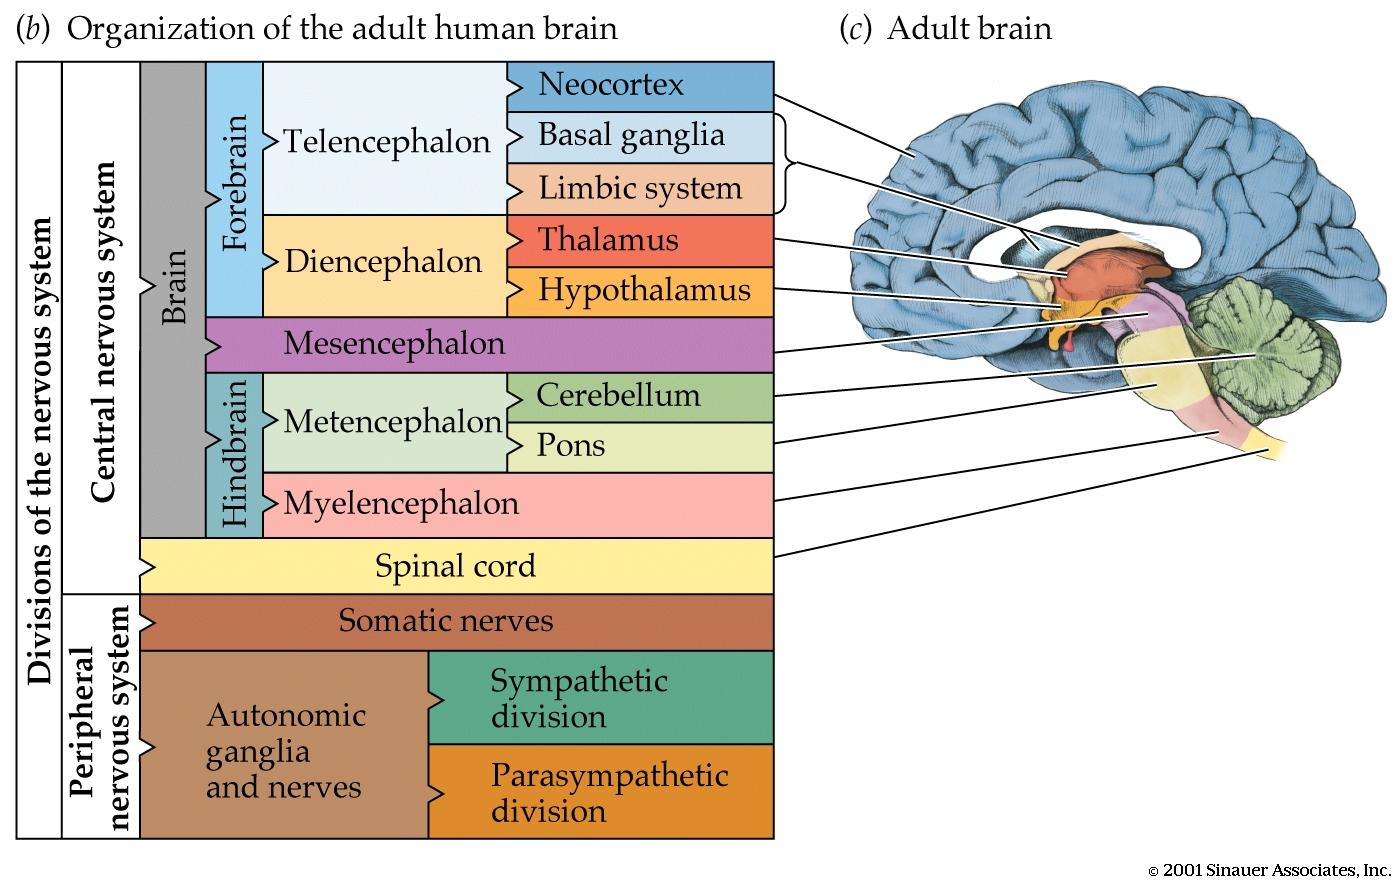
\includegraphics[width=\linewidth]{imgs/division_nervous_system.jpg}
  \caption{Division of the Nervous System}
  \label{fig:nervousSystem}
\end{figure}

\begin{itemize}
\item CNS
\subitem Brain
\subitem Spinal Cord
\item PNS
\subitem Somatic and autonomic nervous system
\end{itemize}

Both system contains gray and white matter.
In the PNS the gray matter contains \textbf{ganglia}: collection of neuron cell
bodies -, the white matter contains \textbf{nerves}: bundles of axons.
In the CNS the gray matter is divided in:
\begin{itemize}
\item Neural cortex - gray matter on the surface of the brain
\item Nuclei - collection of neuron cell bodies in the interior of CNS
\item Centers - collection of neuron cell bodies in CNS, each center has specific processing functions
\item High centers - the most complex centers in brain.
\end{itemize}
The white matter in CNS is divided in two parts: the \textbf{tracts or fasciculus}: bundle of CNS axons
that share a common origin and destination -, and the \textbf{columns or funiculus}: several tracts (fasciculi) that form an anatomically distinct mass

The centers and tracts that connect the brain with other organs and system in
the body are called \textbf{pathways}. The ascending (sensory) pathway is called afferent.
The descending (motor) pathway is called efferent.

Figure \ref{fig:brain} shows the macro division of the brain: Telencephalon, Diencephalon, Brain stem (Midbrain or Mesencephalon, Pons and Cerebellum and Medulla oblongata) and Medulla spinallis), in \ref{fig:brain2} we can see some views of the brain.
Also part of the anatomy of the brain: cranial nerves, meninges, ventricles / cerebrospinal fluid and cerebral circulation.

\begin{figure}
  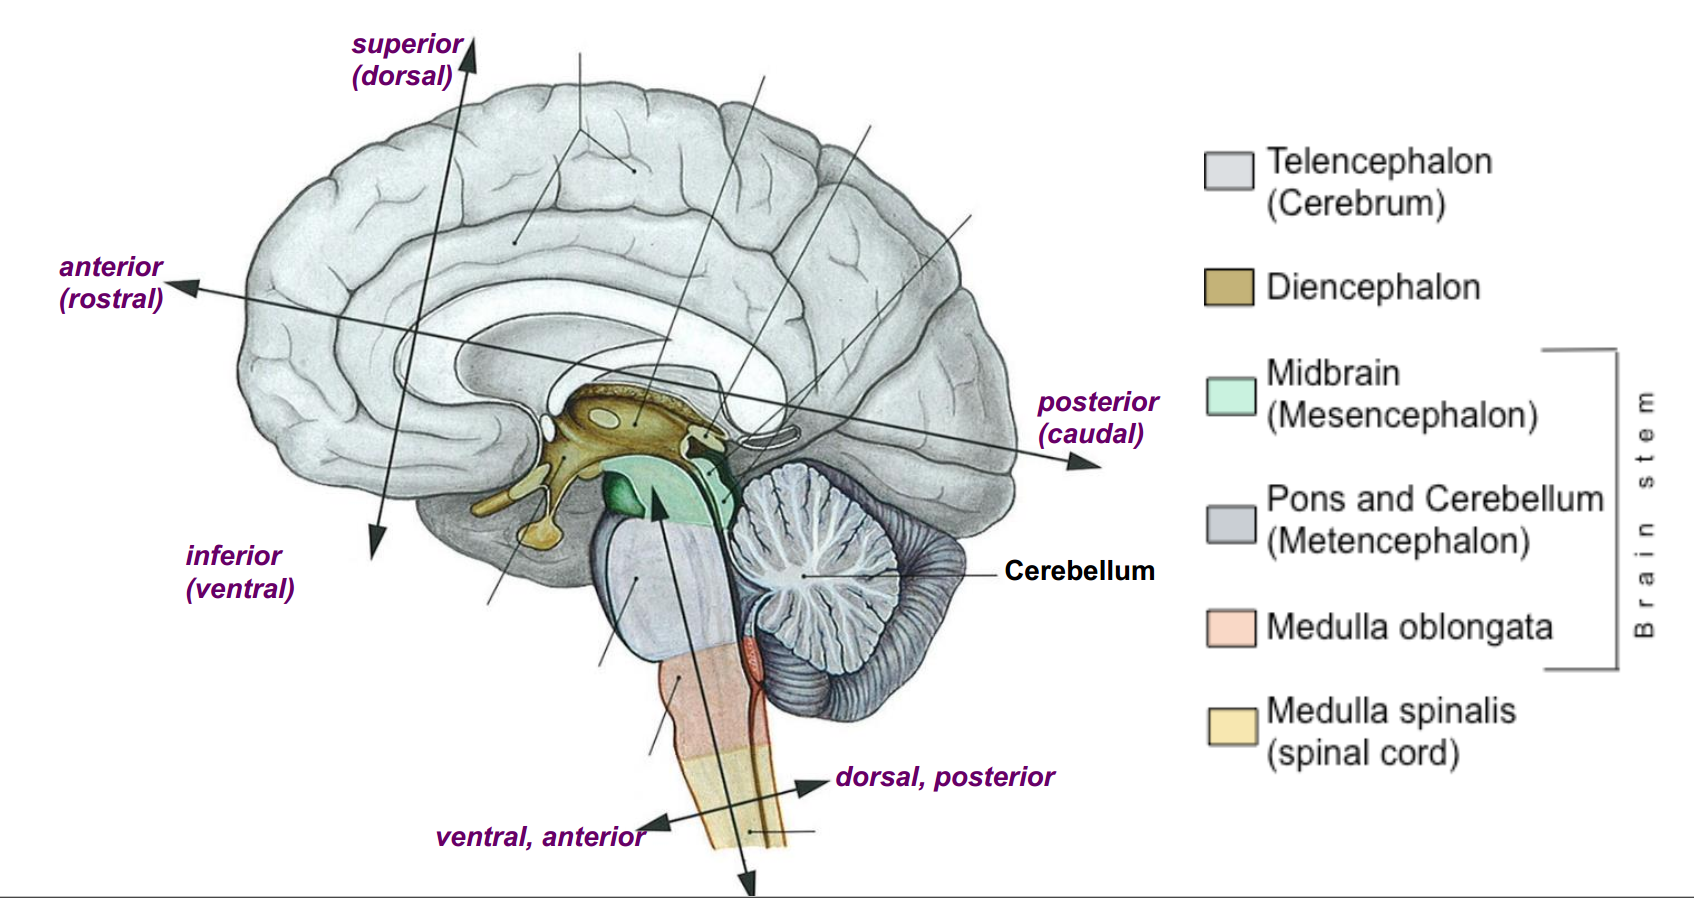
\includegraphics[width=\linewidth]{imgs/viewsOfTheBrain.png}
  \caption{Division of the brain}
  \label{fig:brain}
\end{figure}

\begin{figure}
  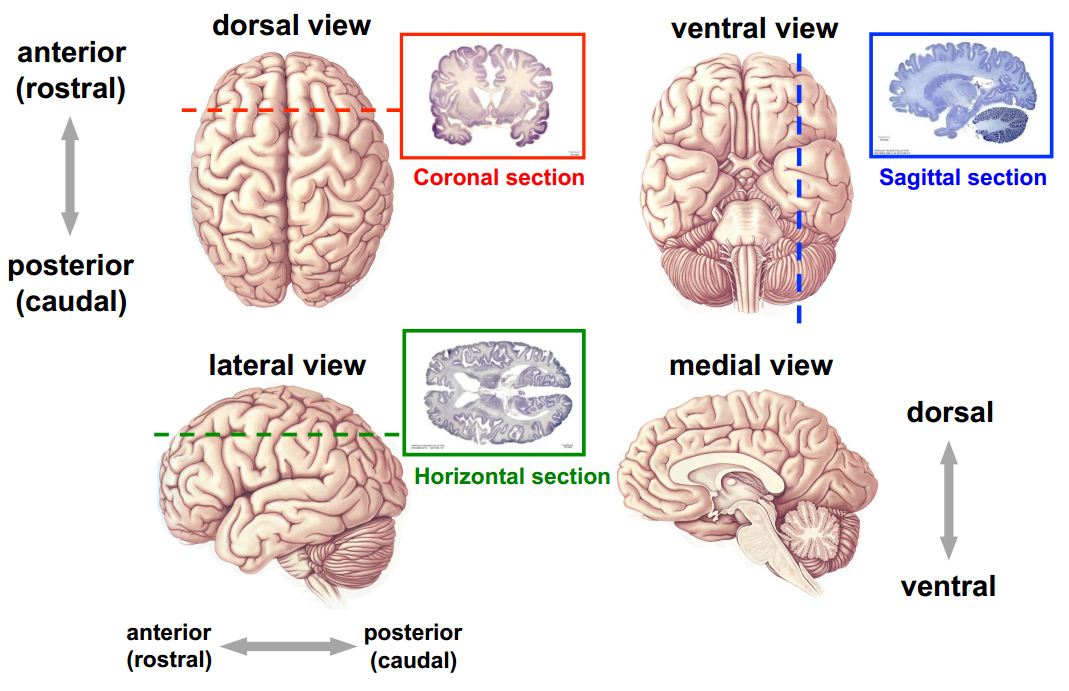
\includegraphics[width=\linewidth]{imgs/viewsOfTheBrain2.png}
  \caption{Views of the Brain}
  \label{fig:brain2}
\end{figure}

\paragraph{Telencephalon - or Forebrain}
The telencephalon (the biggest part of the brain) is divided in lobes, functional cortical areas, basal ganglia and limbic system.

The four lobes (frontal, occitopital, temporal and parietal) are presented in Figure \ref{fig:boundaries}.

\subparagraph{Gray matter}
The macroscopic boundaries of the gray matter are Gyri, Sulci and Commissural fiber tracts. Each one is divided as follows:
\begin{itemize}
\item Gyri
\subitem precentral gyrus
\subitem postcentral gyrus
\subitem pars triangularis
\subitem angular gyrus
\subitem cingulate gyrus
\subitem parahippocampal gyrus
\item Sulci
\subitem central sulcus
\subitem lateral fissure
\subitem parieto-occipital sulcus
\subitem calcarine sulcus
\item Commissural fiber tracts
\subitem corpus callosum
\subsubitem Rostrum
\subsubitem Genu
\subsubitem Truncus
\subsubitem Splenium
\subitem anterior commissure
\end{itemize}

Figure \ref{fig:boundaries} shows the macroscopic boundaries of the gray matter. Besides the anatomical division, there is a functional division of the brain, where each area in the cerebral cortex has specific functional activities. The Wernicke's (language comprehension) and Broca's (speech production) areas are highlited in Figure \ref{fig:functionalBoundaries}.

In 1909 Korbinian Brodmann described areas of the cerebral cortex on the basis of
cytoarchitectural criteria. Areas differ in celltypes, layering and cell distribution, resulting in 52 Brodman Areas.

The human brain is gyrencephalic, i.e, is formed by giri, as the elephant brain. However other species can be  lissencephalic (the brain is smooth, without giri) as the domestic rabbit and the house mouse. Defects in the neuronal migration during early to mid gestation (12th to 24th weeks) leading to impaired development of gyri and sulci.

\begin{figure}
  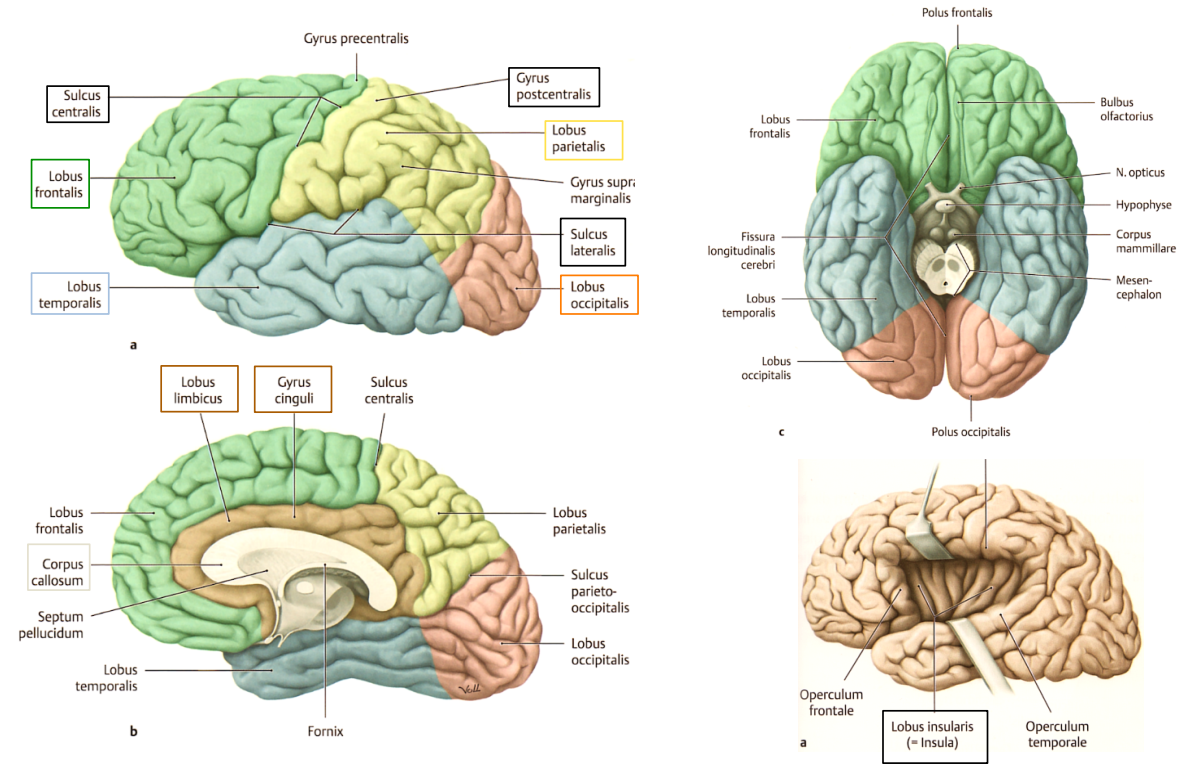
\includegraphics[width=\linewidth]{imgs/macroscopic_boundaries.png}
  \caption{Macroscopic Boundaries - gray matter of the cortex}
  \label{fig:boundaries}
\end{figure}

\begin{figure}
  \centering
  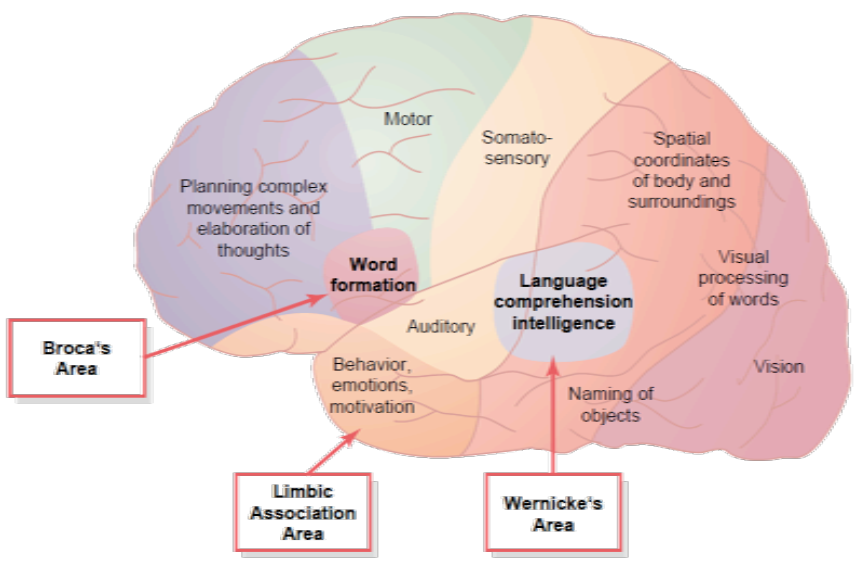
\includegraphics[width=12cm]{imgs/functional_boundaries.png}
  \caption{Functional Division - gray matter of the cortex}
  \label{fig:functionalBoundaries}
\end{figure}

\newpage

\subparagraph{White matter}

\begin{wrapfigure}[11]{r}{0.5\textwidth}
	\centering
  	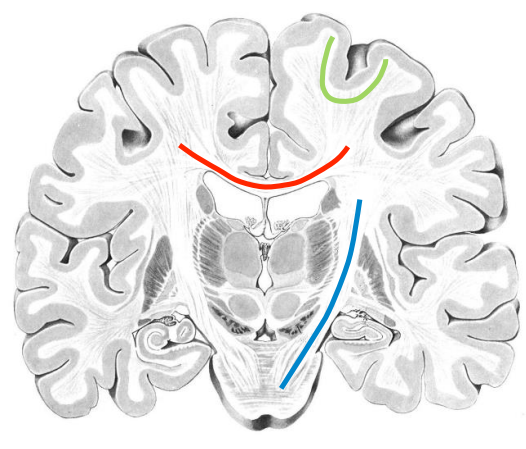
\includegraphics[width=5cm]{imgs/macroscopic_whiteMatter.png}
	\caption{White matter - macroscopic fibers}
  	\label{fig:macroscopic_whiteMatter}
\end{wrapfigure}

The white matter can be divided macroscopically and microscopically. Macroscopically we talk about fibers and microscopically we talk about cells. Figure \ref{fig:macroscopic_whiteMatter} exemplify the macroscopic division and Figure \ref{fig:microscopic_whiteMatter} exemplify the microscopic division, where we can see microglias, astrocyte and oligodendrocytes cells.

\begin{itemize}
\item Comissural fibers (red): link areas between the two hemispheres (corpus callosum, anterior commissure, posterior commissure)
\item Association fibers (green): link cortical areas of the same hemisphere.
\item Projecting fibers (blue): link the cortex with subcortical areas of the brain and the spinal cord.
\end{itemize}

\begin{figure}
  \centering
  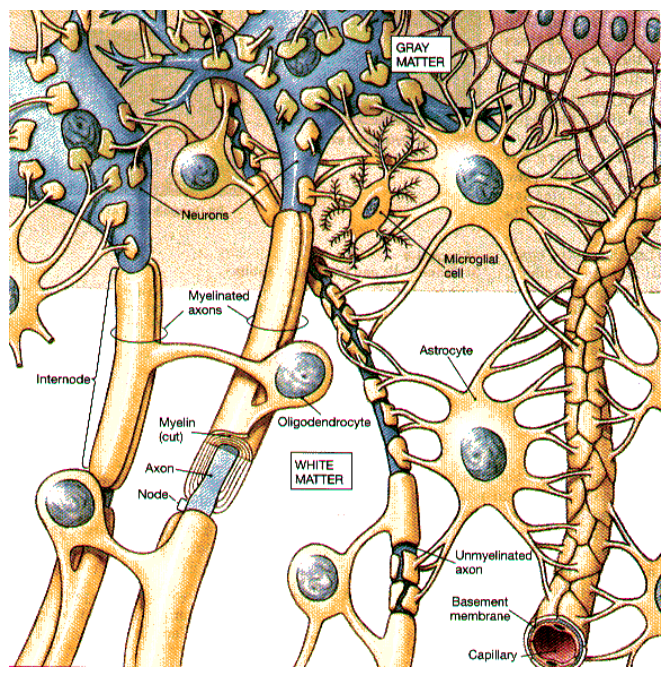
\includegraphics[width=12cm]{imgs/microscopic_whiteMatter.png}
  \caption{White Matter - microscopic structures}
  \label{fig:microscopic_whiteMatter}
\end{figure}

\subparagraph{Basal Ganglia}

The basal ganglia are the principal subcortical components of a family of neuronal circuits which link the thalamus and cerebral cortex. It is crucial for the initiation and modulation of voluntary movement by sending their output to the motor cortex via the thalamus. In addition, the basal ganglia also contribute to a variety of behavioral and cognitive functions other than voluntary movement.

The basal ganglia is divided in:
\begin{itemize}
\item Striatum: is the major recipient of inputs from the substantia nigra, cerebral cortex, thalamus, and brain stem. In humans (and most primates) consist of the caudate nucleus, the putamen, and the nucleus accumbens. In rats and mices consist of caudate putamen (human caudate nucleus + putamen) and nucleus accumbens.
\item Globus Palidus: is divided into external and internal segments.
\subitem The internal segment (GPi) sends projections to the thalamus and pedunculopontine nucleus (a group of cells located in the brain stem).
\subitem The external segment (GPe) sends projections to the internal segment of the globus pallidus and to the subthalamic nucleus.
\item Susbtantia Nigra: is a midbrain (mesencephalon) structure and contains a dense population of dopamine cells. The substantia nigra can be subdivided into substantia nigra pars compacta and pars reticulata.
\end{itemize}

One of the disorders of the basal ganglia is the parkinson's disease, where the dopaminergic cells in the substantia nigra pars compacta are lost, it impairs motor skills, speech and other functions.

\subparagraph{Limbic system}
Divided in cingulate gyrus (superior portion of limbic lobe), parahippocampal gyrus (inferior portion of limbic lobe), hippocampus and amigdalar complex.
In Alzheimer's disease, the hippocampus is one of the first regions of the brain to suffer damage. memory problems (especially spatial memories) and disorientation appear among the first symptoms. People with extensive, bilateral hippocampal damage (such as in patients with progressed AD) may experience anterograde amnesia (the inability to form or retain new memories).
The amigdala is envolved in emotions.

\paragraph{Diencephalon}
The diencephalon is divided in thalamus, hipothalamus, epithalamus, subthalamus

\subparagraph{Thalamus}
The thalamus is the gatekeeper of the brain: it is important for the transfer of information from the periphery to sensory processing regions in the telencephalon. It has important gating (filtering) functions: it determines whether sensory information reaches conscious awareness in the neocortex and participates in the integration of motor information from the cerebellum and basal ganglia and transmits this information to cerebral areas concerned with movement.

\subparagraph{Hipothalamus}
The hipothalamus regulates several behaviors that are essential for homeostasis
and reproduction: growth, eating, drinking and maternal behavior, by regulating hormonal secretions from the pituitary gland. It is an important control center for the autonomic nervous system and for the hypothalamus-pituitary-adrenal (HPA) stress-response system.

\subparagraph{Neuroendocrinollogy of Hipothalamus}
\begin{enumerate}
\item Hipothalamus produces releasing hormones (rh) and inhibiting hormones (ih) that directly influence anterior pituitary hormone secretion.
\item Hipothalamus produces two hormones (oxytocin and antidiuretic hormone) that are stored in the posterior pituitary.
\item Hupothalamus overseesthe ANS (?)thereby helping to stimulate the adrenal medulla via sympathetic innervation.
\end{enumerate}

\subparagraph{Epithalamus}
epithelial roof of the third ventricle, habenula, pineal body and afferent/efferent connections. It is responsible for the secretion of melatonin, regulation of day-night cycles, information processing related to olfaction.

\subparagraph{Subthalamus}
It is the continuation of the tegmentum. Functionally part of the basal ganglia (motor control).

\newpage

\paragraph{Mesencephalon - or Midbrain}
\begin{wrapfigure}[11]{r}{0.5\textwidth}
	\centering
  	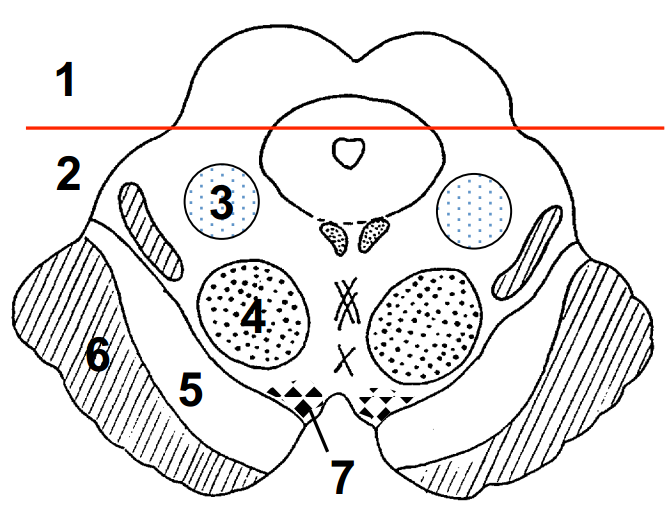
\includegraphics[width=7cm]{imgs/mesencephalon.png}
	\caption{Mesencephalon - Functional units}
  	\label{fig:mesencephalon}
\end{wrapfigure}

The midbrain is a portion of the CNS associated with vision, hearing, motor control, sleep/wake, arousal (alertness), and temperature regulation. It comprises the tectum (or corpora quadrigemina), tegmentum, the cerebral aqueduct (or ventricular mesocoelia or "iter"), and the cerebral peduncles, as well as several nuclei and fasciculi. Caudally the midbrain adjoins the metencephalon (afterbrain) (pons and cerebellum). while rostrally it adjoins the diencephalon (thalamus, hypothalamus, etc). In Figure  \ref{fig:mesencephalon} the parts of the midbrain are listed.

\begin{enumerate}
\item Tectum (roof)
\subitem superior colliculus: visual and occulomotor reflexes
\subitem inferior colliculus: relay auditory tract
\item Tegmentum (floor)
\item Reticular formation: automatic processing of incoming sensation and outgoing motor
commands, helps to maintain consciousness, can initiate motor response to stimuli (see also
medulla oblongata!)
\item Red nucleus: involuntary control of background muscle tone and limb posture
\item Substantia nigra: regulates activity in the basal nuclei, degeneration of dopaminergic cells causes Parkinson’s disease
\item Cerebral peduncles: connect primary motor cortex with motor neurons in brain and spinal cord, carry ascending sensory information to thalamus
\item Ventral tegmental area (VTA): part of the limbic system, projects e.g. to nucleus accumbens and amygdala, emotional reinforcement.
\end{enumerate}

\paragraph{Pons}
\begin{wrapfigure}[7]{r}{0.5\textwidth}
	\centering
  	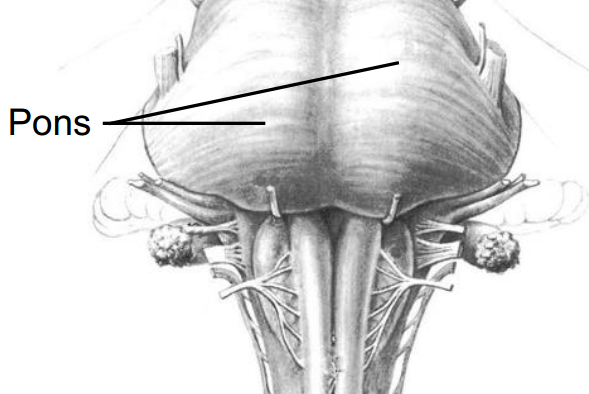
\includegraphics[width=7cm]{imgs/pons.png}
	\caption{Pons}
  	\label{fig:mesencephalon}
\end{wrapfigure}

Divded in two parts: locus coeruleus and pontine nuclei. The locus coeruleus (or blue spot) contains noradrenergic cells innervating large portions of the brain, mediating physiological response to panic and stress. The pontine nuclei receive fibers from all cortical areas and relay to the contralateral cerebellum.

\paragraph{Medulla oblongata}
\begin{figure}
	\centering
  	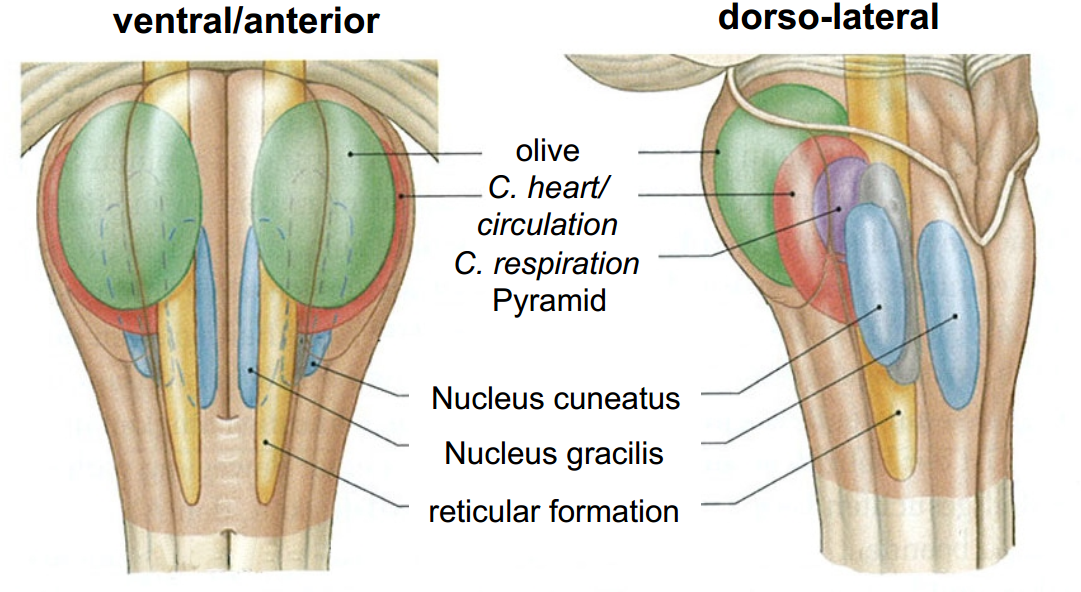
\includegraphics[width=\linewidth]{imgs/medullaOblongata.png}
	\caption{Medulla Oblongata}
  	\label{fig:medullaOblongata}
\end{figure}

It contains four main parts: olives, pyramid, reticular formation and reflex centers.\subparagraph{olive} relay nucleus for afferent connection from motor cortex and red nucleus, efferent to contralateral cerebellum.
\subparagraph{pyramid} contains descending cortico-spinal fibers.
\subparagraph{reticular formation (entire brain stem!)} containing the raphe nuclei and magno/parvocellular nuclei, which regulate respiration, circulation, vomiting, swallowing, and pain control.
\subparagraph{reflex centers} for heart and circulation (vasomotor/cardiac) and
respiratory rhythmicity.

\paragraph{Cerebellum}
\begin{figure}[H]
	\centering
  	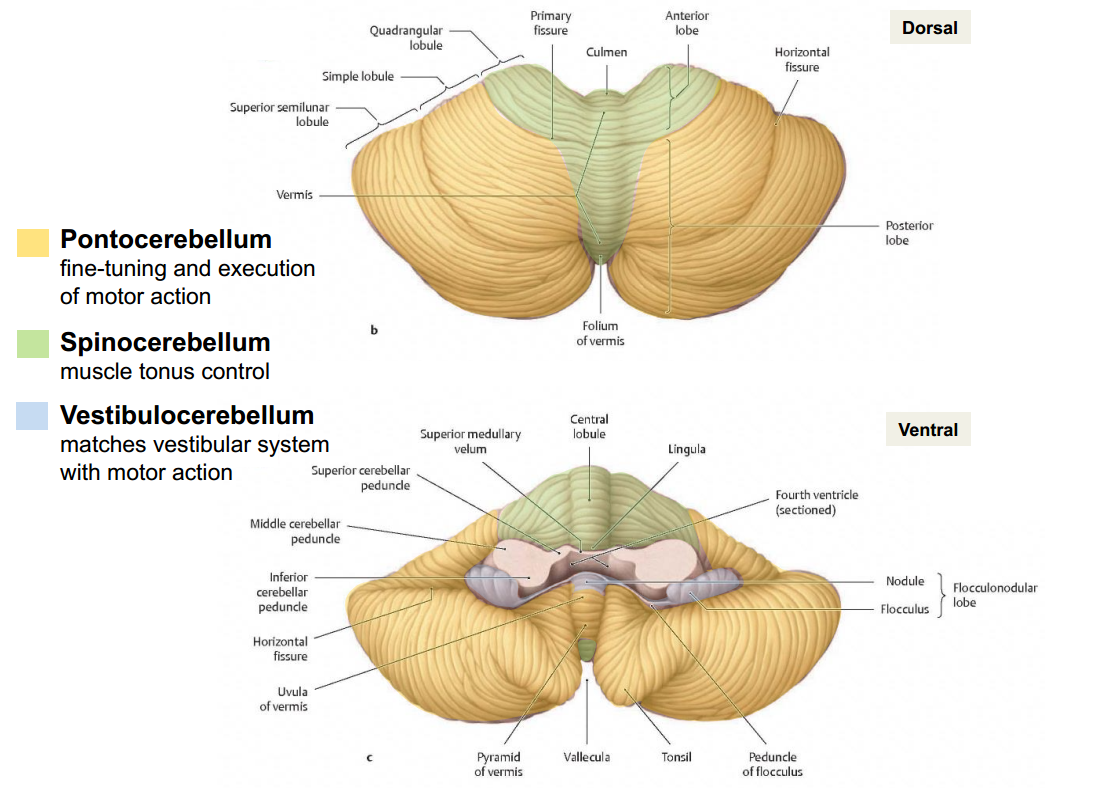
\includegraphics[width=\linewidth]{imgs/cerebellum.png}
	\caption{Cerebellum}
  	\label{fig:cerebellum}
\end{figure}

\paragraph{Spinal Cord}
\begin{figure}
	\centering
  	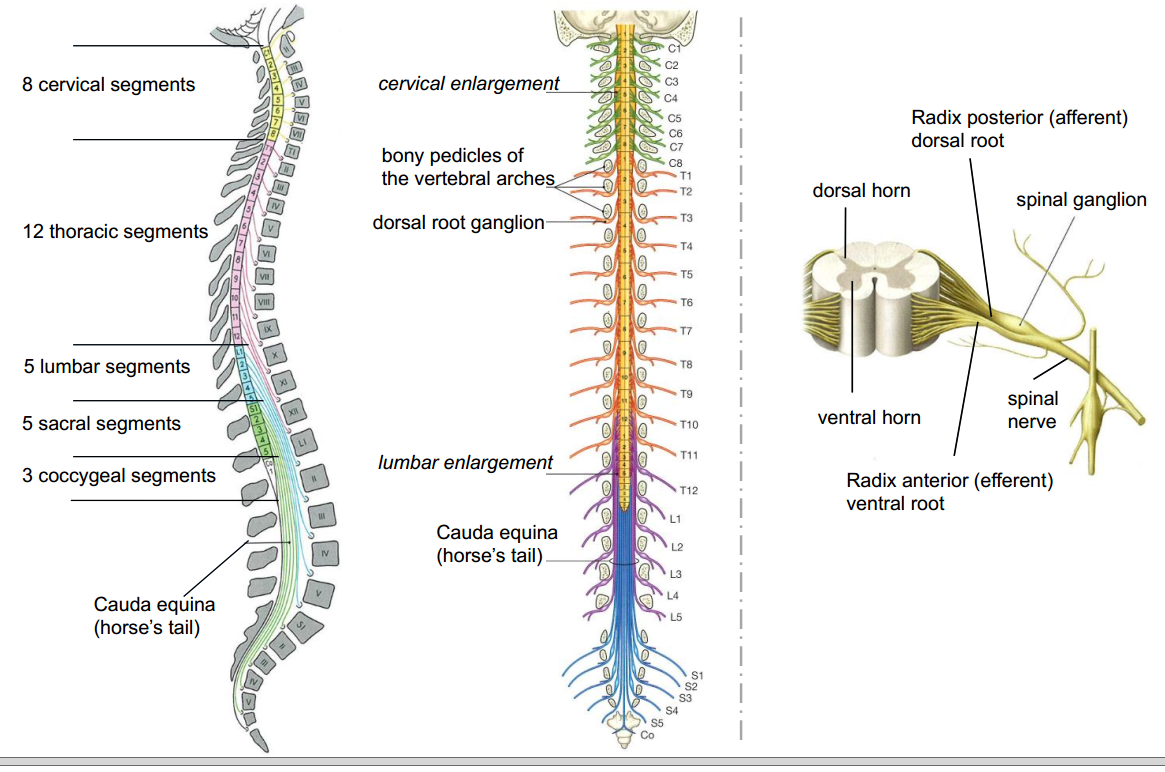
\includegraphics[width=\linewidth]{imgs/spinalCord.png}
	\caption{Spinal Cord}
  	\label{fig:spinalCord}
\end{figure}

The segmental organization of the spinal cord is ilustrated in Figure \ref{fig:spinalCord}. The spinal cord contains gray and white matter. 
The gray matter (inside part) of the spinal  cord consists of cell bodies of interneurons, motor neurons, and synaptic connections. Fibers of the motor neurons in the ventral horn leave the spinal cord to muscles (efferent/motor commands). Afferent/sensory axons enter through the dorsal horn and either synapse on sensory interneurons in the dorsal horn, or join the ascending tracts in the white matter.
The white matter of the spinal cord mostly consists of myelinated axons of motor and sensory neurons organized in columns (containing several fiber tracts) carrying information to (afferent/ascending) and from (efferent/descending) the brain.

\paragraph{Cranial Nerves}
Cranial nerves are the nerves that emerge directly from the brain (mostly from the
brainstem), in contrast to spinal nerves (which emerge from segments of the spinal cord).
Cranial nerves are generally named according to their structure or function. We have 12 cranial nerves: (i) olfactory, (ii) optical, (iii) oculomotor, (iv) trochlear, (v) trigeminal, (vi) abducens, (vii) facial, (viii) vestibulocochlear, (ix) glossopharyngeal, (x) vagus, (xi) accessory and (xii) hypoglossal nerve as we can see in Figure \ref{fig:cranialNerves}.
\begin{figure}
	\centering
  	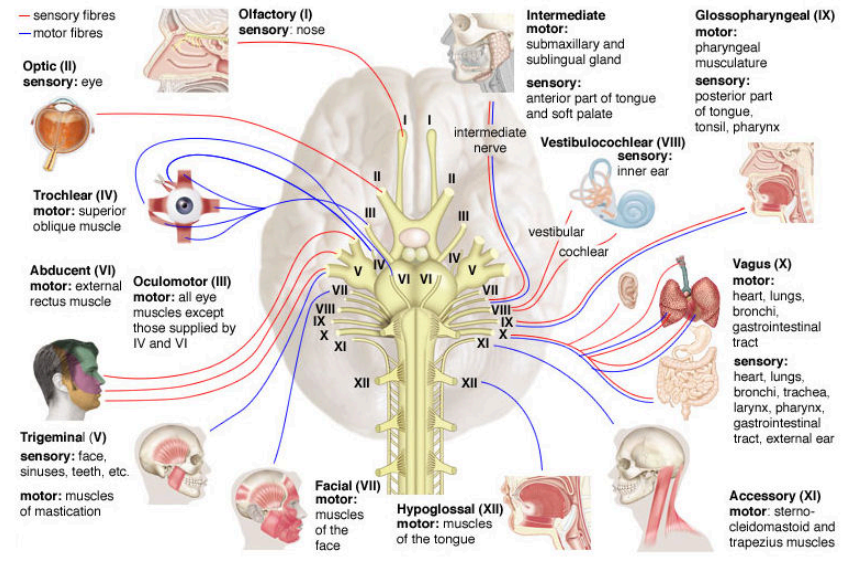
\includegraphics[width=\linewidth]{imgs/cranialNerves.png}
	\caption{Cranial Nerves}
  	\label{fig:cranialNerves}
\end{figure}

The cranial nerves provide motor and sensory innervation mainly to the structures within the head and neck. The sensory innervation includes sensation such as temperature and touch, and innervation such as taste, vision, smell, balance and hearing. The vagus nerve (x) provides sensory and autonomic (parasympatheic) innervation to most of the organs in the chest and abdomen.

\paragraph{Meninges}
The meninges are the three membranes that envelop the brain and spinal cord. In mammals, the meninges are the \textbf{dura mater}, the \textbf{arachnoid mater}, and the \textbf{pia mater}. The inflamation of the meninges is called Meningitis.
\begin{itemize}
\item Dura mater: leather-like, inflexible layer surrounding the CNS and spinal cord. Inner and outer layers, containing large venous sinuses (e.g. superior sagittal sinus).
\item Arachnoid mater: loose connective tissue bridging the liquor-filled space (subarachnoidal space) between dura mater and pia mater. Contains all larger blood vessels.
\item Pia mater: translucent, thin membrane directly covering the entire surface of the brain, follows all sulci and gyri.
\end{itemize}

\paragraph{Ventricles and cerebrospinal fluid}
\begin{figure}
	\centering
  	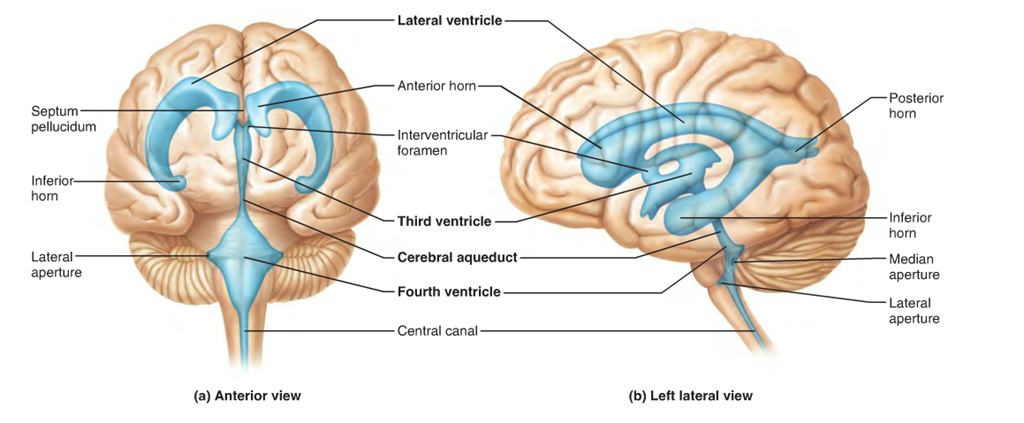
\includegraphics[width=\linewidth]{imgs/ventricles-of-brain.png}
	\caption{Ventricles}
  	\label{fig:cranialNerves}
\end{figure}
The ventricles of the brain are a communicating network of cavities filled with cerebrospinal fluid (CSF) and located within the brain parenchyma. The ventricular system is composed of 2 lateral ventricles, the third ventricle, the cerebral aqueduct, and the fourth ventricle.
Some disorders on the ventricles cause diseases: neurodevelopmental (schizophrenia), neurodegenerative (alzheimer).

CSF is clear fluid, high content of NaCl, contains glucose and K+, low in proteins, very few cells (lymphocytes). It turnover three times a day. It flows throughout the ventricular system and is absorbed back into the bloodstream (via bloodbrain-barrier).
Cerebrospinal fluid is located in the subarachnoid space between the arachnoid mater and the pia mater.

\subparagraph{Functions of CSF} Buoyancy, Protection and Homeostasis. \\
\textbf{Buoyancy}: The actual mass of the human brain is approx. 1500 grams; however, the net weight of the brain suspended in the CSF is equivalent to a mass of 25 grams. The brain therefore exists in neutral buoyancy, which allows the brain to maintain its density without being impaired by its own weight, which would cut off blood supply. \\
\textbf{Protection}: CSF protects the brain tissue from injury when jolted or hit. In addition, it helps regulating intracranial pressure (lowering CSF production can help preventing brain ischemia). \\
\textbf{Homeostasis}: Through absorption back into the blood stream, CSF can rinse “metabolic waste” from the CNS, allowing for a homeostatic regulation of the brain. \\
Commont related pathology: hidrocephalus - abnormal accumulation of CSF within the brain. Can be congenital or acquired postnatally. Most common cause is aqueductal stenosis (passage between the 3rd and 4th ventricle is blocked or to narrow), so fluid accumulates in the upper ventricles.

\paragraph{Cerebral circulation}
The brain is one of the most metabolically active organs in the body! Uses approximately 20-25\% of the body’s total energy requirements (despite accounting for only 2\% of the body’s mass). The brain stores little energy as glycogen and relies mostly on circulating glucose. The rate of the cerebral blood flow in the adult is typically 750 milliliters per minute, representing 15\% of the cardiac output.

\subparagraph{Arteries} Supply oxygen-rich blood from heart to brain. Main branches of the internal carotids: anterior cerebral artery and middle cerebral artery. Main branches of the vertebral / basilar arteries: 3 arteries supplying the cerebellum and posterior cerebral artery.
\subparagraph{Veins} Carry oxigen-depleted blood away from brain

\begin{figure}
	\centering
  	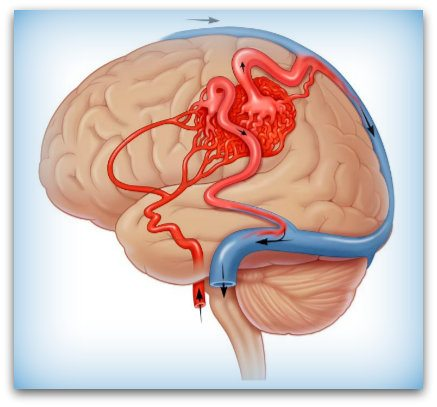
\includegraphics[width=10cm]{imgs/avm_large.jpg}
	\caption{Arteries and Veins of the Brain}
  	\label{fig:arteriesVeinsBrain}
\end{figure}

\subsection{Comparative Neuroanatomy}

\subsubsection{Does brain size matter?}
\begin{figure}
	\centering
  	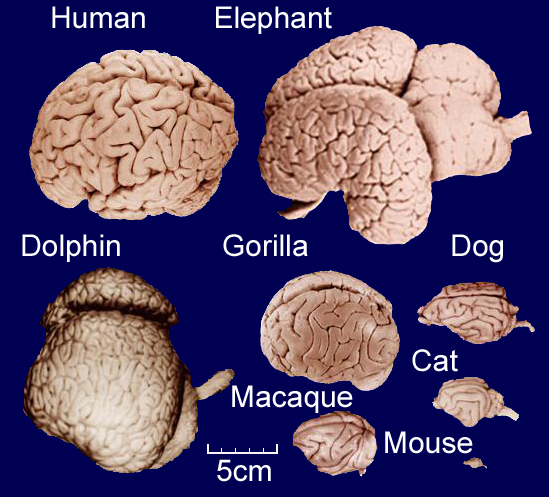
\includegraphics[width=10cm]{imgs/comparativeBrainSize.jpg}
	\caption{Brain size of different species}
  	\label{fig:comparativeBrainSizes}
\end{figure}

Is there a relationship between the size of an animal's brain and some kind of “behavioural complexity”? Not really. Elephants and whales have brains 4 to 5 times the size of a human being's, yet their behaviour is generally agreed to be less complex than ours.

\paragraph{Encephalization Quotient (EQ)} describes brain size as a ratio of the expected average brain size relative to the actual body weight. EQ of humans: $\approx$ 7.5 (Human brains are 7.5x bigger than what one would expect for species of this size.) EQ of sq. monkeys: $\approx$ 1.1.

\paragraph{Body mass and number of neurons} A capybara has 1,600,000,000 neurons and a common squirrel monkey (much smaller than a capybara) has 3,246,000,000 neurons.

\subsubsection{Brain evolution in view of cortical expansion}
Cortical expansion is often equated with "brain evolution”, whereby the relative size of the cerebral cortex increases while the relative size of the cerebellum remains fairly constant. We can see in Figure \ref{fig:corticalExpansion} the human cortical expansion is relative but does not affect each region simirlaly.

\begin{figure}
	\centering
  	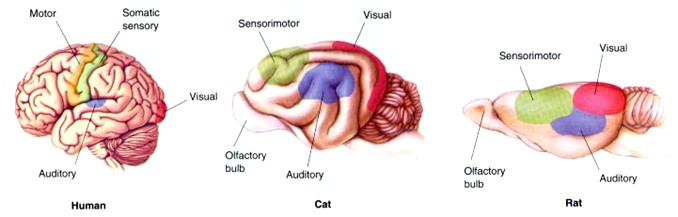
\includegraphics[width=\linewidth]{imgs/comparativeNeuroanatomy.jpg}
	\caption{Cortical expansion}
  	\label{fig:corticalExpansion}
\end{figure}

\subsubsection{Cross-species comparison of cortical areas}

The human prefrontal cortex is responsible for planning, atention, working memory, cognitive flexibility and impulsivity. The human PFC is divided in dorsolateral PFC, anterior cingulate cortex and anterior PFC (or medial PFC). Rats (and mice) also have PFC, with similar responsabilities: lesions to the medial parte of PFC (mPfc) lead to working memory impairements as evident by the \textbf{increased number of working	memory errors in the 8-arm radial arm maze}.
\\
The rodent prefrontal cortex (PFC) is not as anatomically complex as the primate; however,
many of the critical neuroanatomical and functional characteristics are preserved in
rodents, which allow meaningful cross species comparisons relevant to study of the
neurocognitive and neurobiological mechanisms that underlie changes in executive
functioning across the lifespan. The medial portion of rodent PFC [which includes anterior cingulate (aCg), prelimbic (PL), and infralimbic (IL) cortices] shares strong anatomical homology with primate dorsolateral PFC

\subsubsection{Cross-species comparison of subcortical areas}
\begin{figure}[H]
	\centering
  	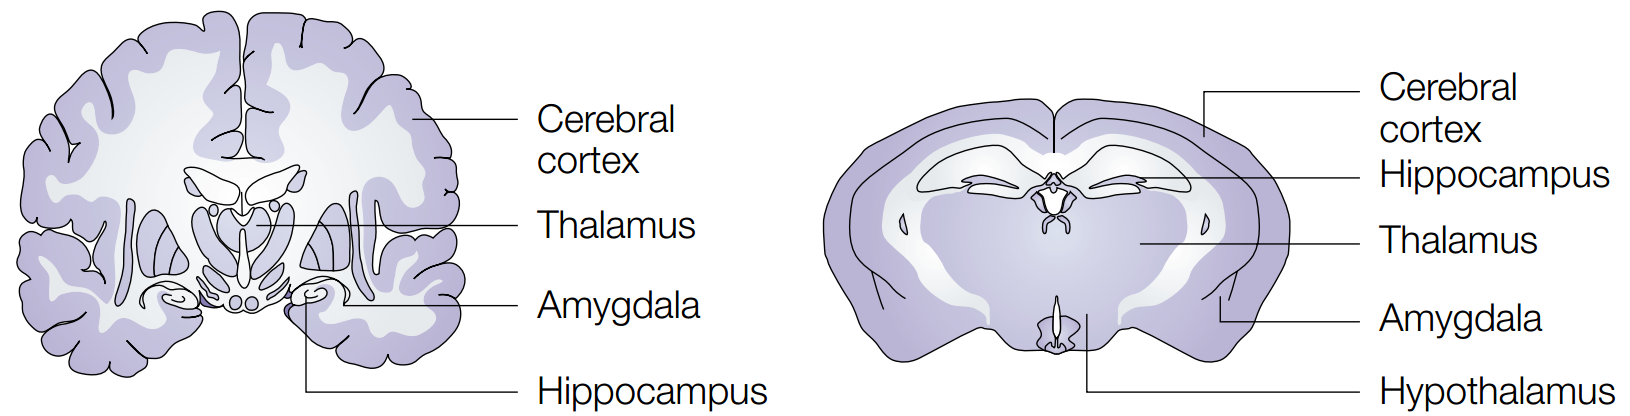
\includegraphics[width=\linewidth]{imgs/subcorticalAreas.png}
	\caption{Cross-species comparison of subcortical areas}
  	\label{fig:subcorticalAreas}
\end{figure}
	
\paragraph{Hippocampus}

\subparagraph{Hippocampal anatomy} The longitudinal axis of the hippocampus is described as ventrodorsal in rodents and as anteroposterior in primates. A rotation of 90-degree is required for the rat hippocampus to have the same orientation as that of primates, as you can see on Figure \ref{fig:hippocampusAnatomy}.
\begin{figure}[H]
	\centering
  	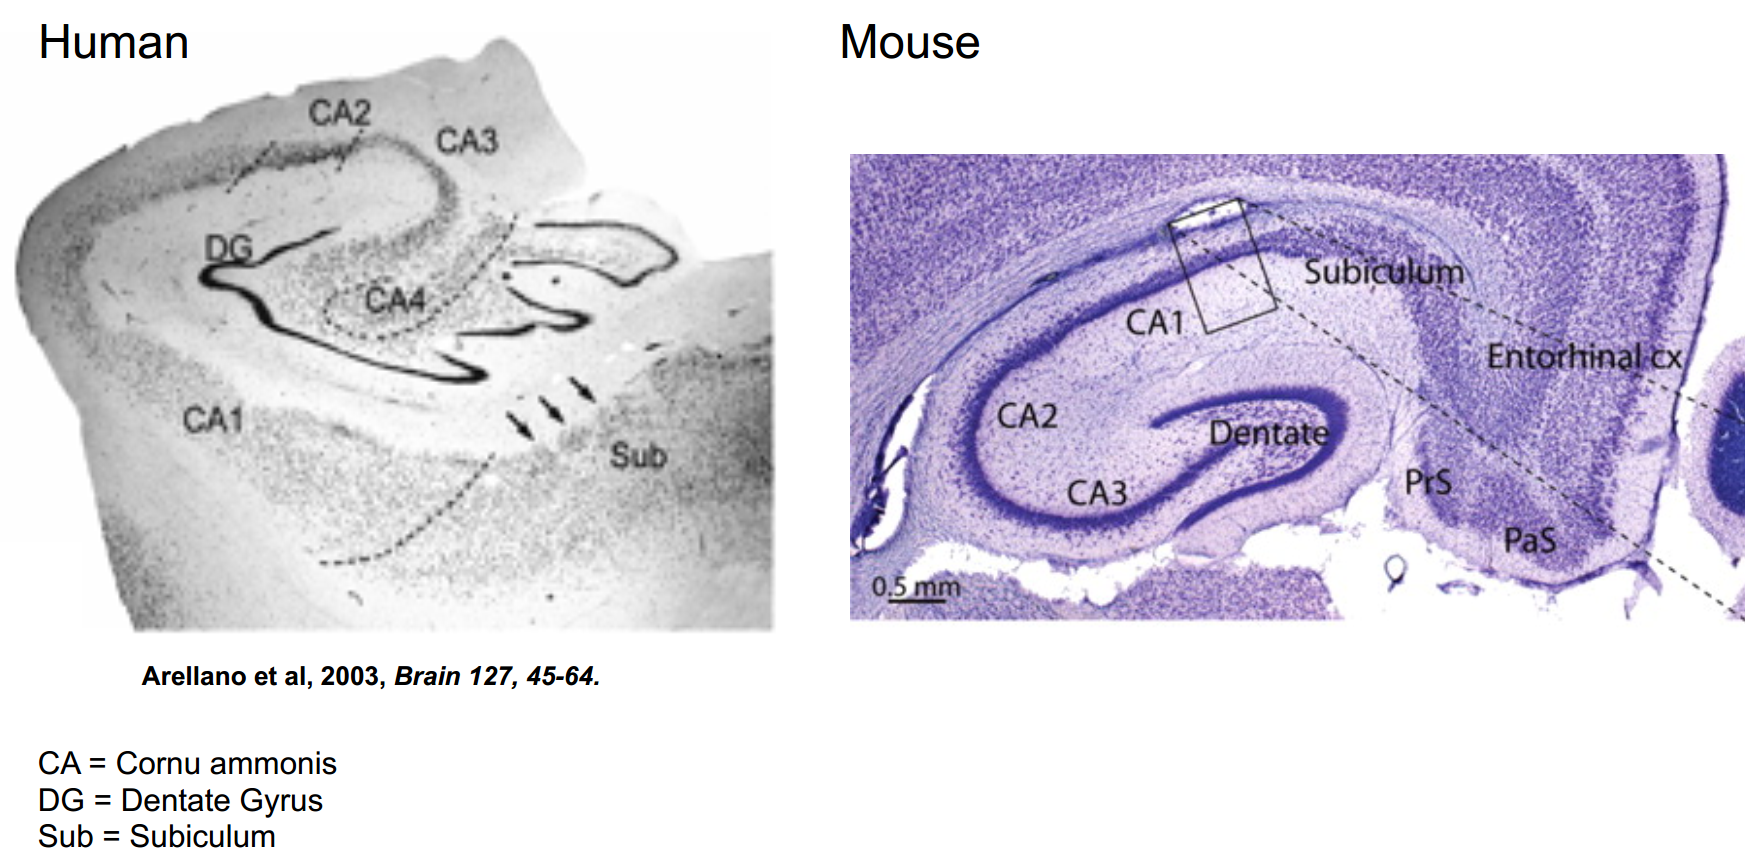
\includegraphics[width=\linewidth]{imgs/cross-species-hippocampus-anatomy.png}
	\caption{Cross-species hyppocampus anatomy}
  	\label{fig:hippocampusAnatomy}
\end{figure}

\subparagraph{Hippocampal Functions} In London taxi drivers were observed an increased brain activity associated with spatial navigation in the \textbf{right hippocampus} and left tail of the caudate. In rats the effect of hippocampal lesions on reference learning and memory was tested using the Morris water maze experiment. As bigger is the lesion on dorsal hippocampall, as bigger the deficit in the acquisition of spatial reference. Not so big deficit if the lesion were in the ventral hippocampal.

Experiment: The position of a submerged platform is constant from trial to trial at a given test day as well as form test day to test day. Animals are repeatedly placed into the tank with varying starting positions; with the help of spatial distal cues as reference points, they are required to find the invisible platform. Following completion of the acquisition phase, the platform is removed from the tank. The animals are once again placed in the tank; the critical measure here is whether the animals would “remember” the position of the platform and therefore would spent more time in quadrant where the platform was positioned before.

\paragraph{Amygdala}

\subparagraph{Amygdalar Anatomy} Primary amygdalar nuclei and basic circuit connections and
function are conserved across species. An enlarged image of the basolateral complex of the
amygdala (BLA) and central nucleus of the amygdala (CeA) or analogues are shown next to a coronalsection from the brains of a lizard, rat, cat, monkey, and human, in Figure \ref{fig:amygdalaAnatomy}.

\begin{figure}
	\centering
  	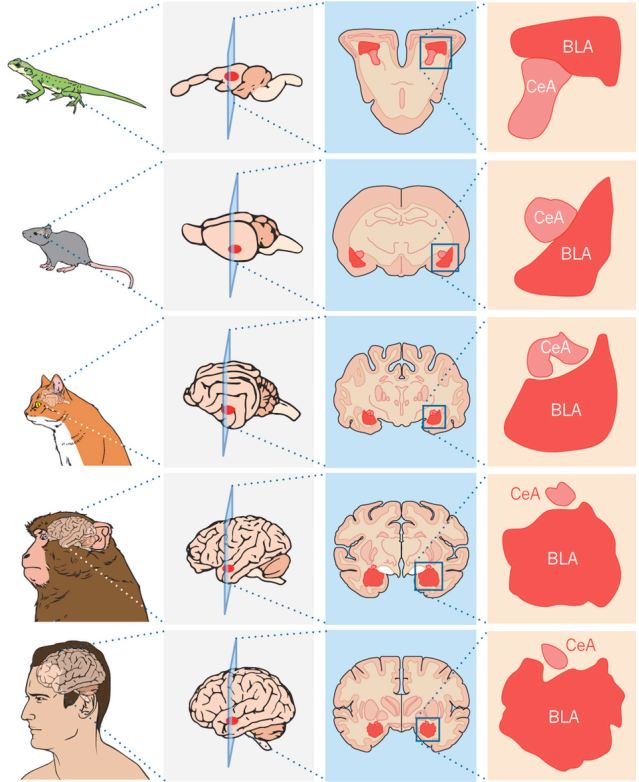
\includegraphics[width=\linewidth]{imgs/amygdalar-anatomy.png}
	\caption{Cross-species amygdalar anatomy}
  	\label{fig:amygdalaAnatomy}
\end{figure}

\subparagraph{Amygdalar Functions} In post-traumatic stress disorders (PTST), the amygdala is hyperactive in response to negative emotional stimulli vs. neutral and positive stimulli. In rodents the investigation of amygdalar function is tested using the \textbf{classical (pavlovian) fear conditioning}. In rats with amygdala lesions, the response to the non-threatening doesn't happen anymore.

Experiment: present a non-threatening stimulus (like a sound) with a noxius stimulus (like a midle shock) until the animal shows a fear response not just to the shock but also to the sound alone.

\paragraph{Basal ganglia}

\subsection{Exercises}

\subsubsection{Coronal section - I}
\begin{figure}[H]
	\centering
  	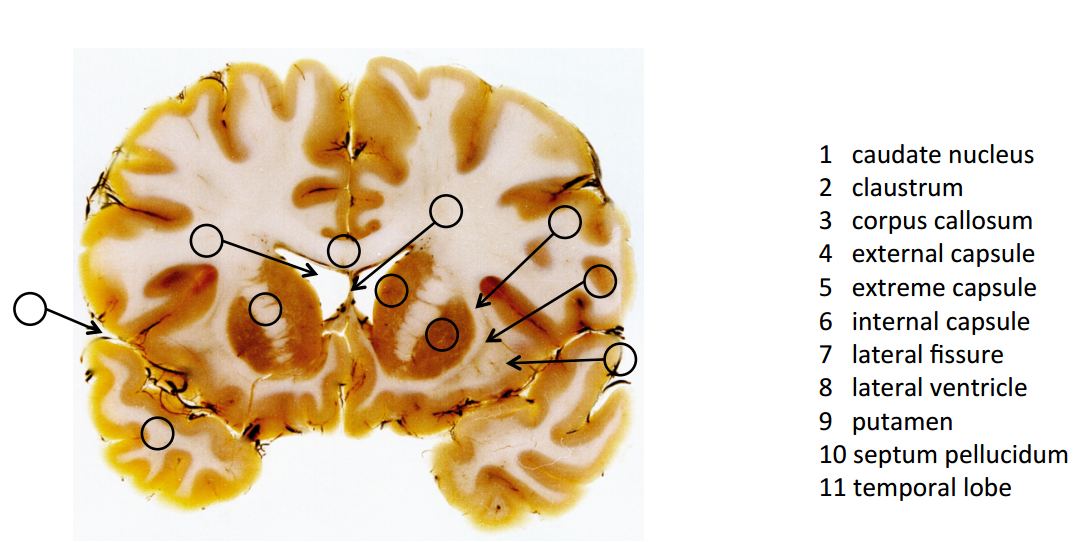
\includegraphics[width=\linewidth]{imgs/coronal-section-I.png}
	\caption{Coronal section I}
  	\label{fig:coronalSectionI}
\end{figure}

\subsubsection{Coronal section - II}
\begin{figure}[H]
	\centering
  	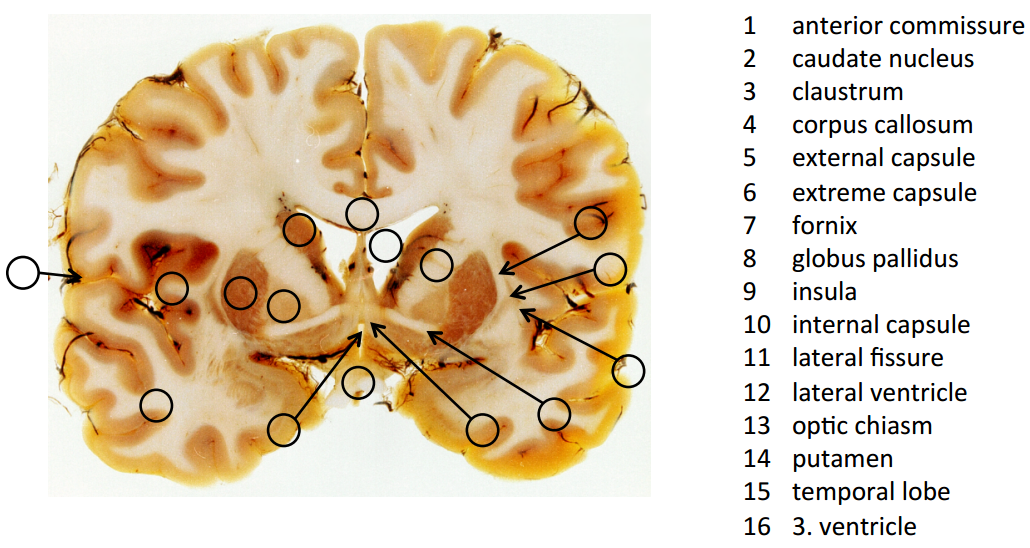
\includegraphics[width=\linewidth]{imgs/coronal-section-II.png}
	\caption{Coronal section II}
  	\label{fig:coronalSectionII}
\end{figure}

\subsubsection{Coronal section - III}
\begin{figure}[H]
	\centering
  	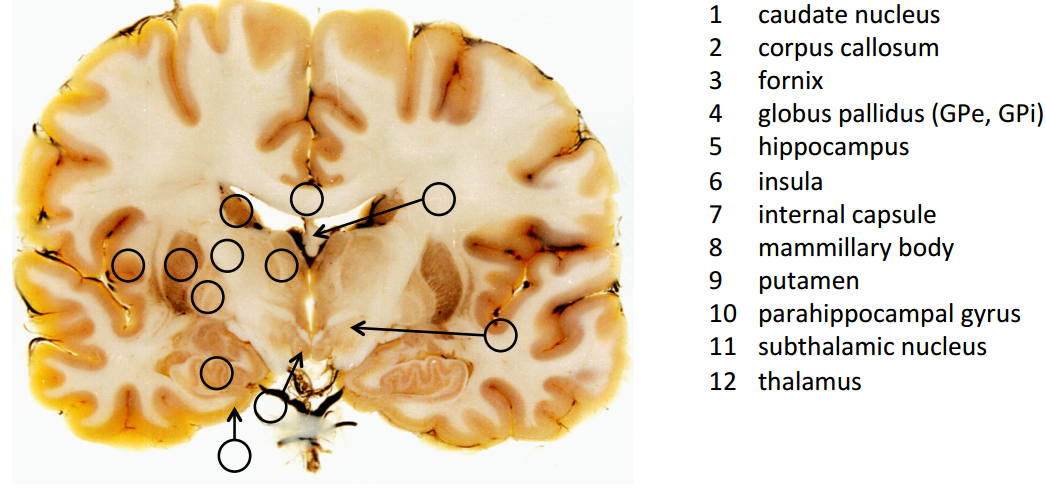
\includegraphics[width=\linewidth]{imgs/coronal-section-III.png}
	\caption{Coronal section III}
  	\label{fig:coronalSectionIII}
\end{figure}

\subsubsection{Coronal section - IV}
\begin{figure}[H]
	\centering
  	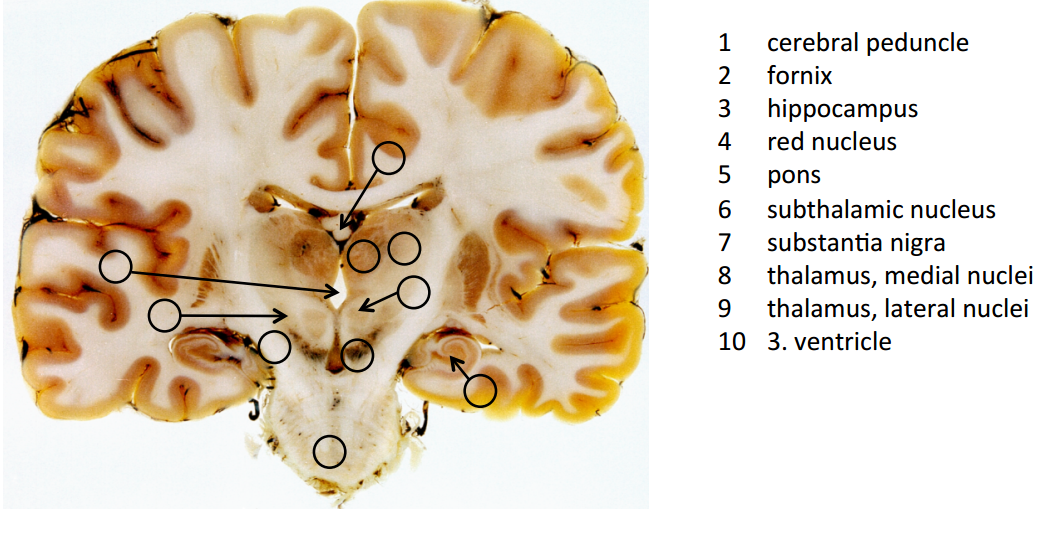
\includegraphics[width=\linewidth]{imgs/coronal-section-IV.png}
	\caption{Coronal section IV}
  	\label{fig:coronalSectionIV}
\end{figure}

\subsubsection{Horizontal section}
\begin{figure}[H]
	\centering
  	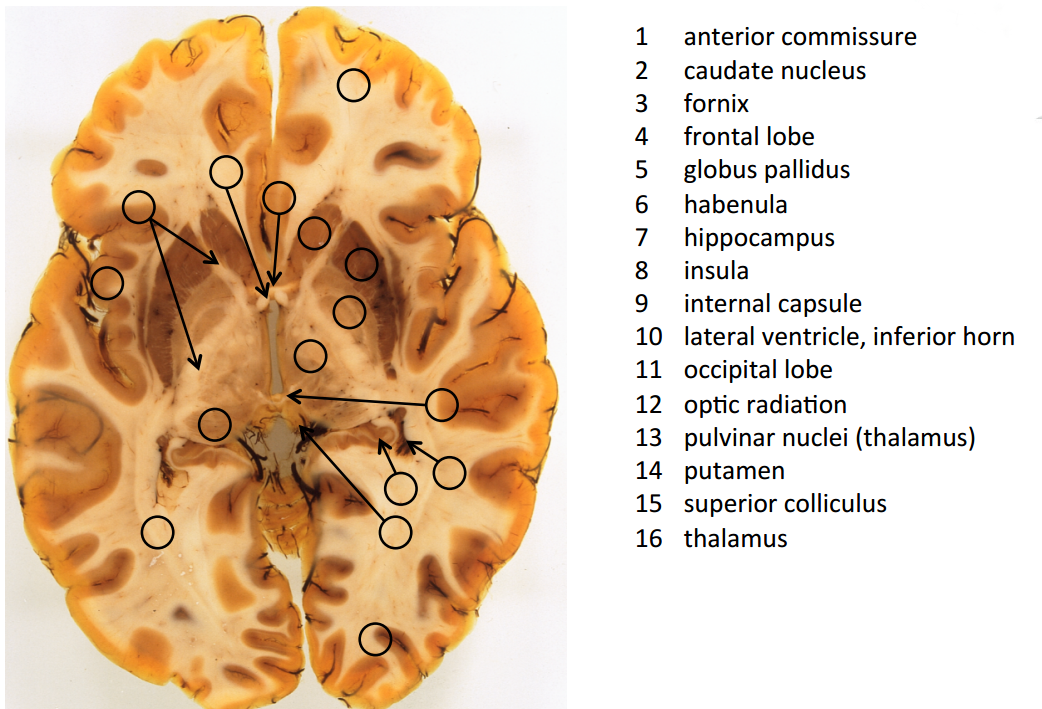
\includegraphics[width=\linewidth]{imgs/horizontal-section.png}
	\caption{Horizontal section}
  	\label{fig:horizontalSection}
\end{figure}

\section{Molecular \& Cellular Neuroscience}
\subsection{Building a central nervous system}
Human brain: 86 billions neurons and about equal number of glia cells.

\subsubsection{Neural Induction and Pattern Formation}

\paragraph{Embryonic Origins of the Nervous System}

\begin{figure}
	\centering
  	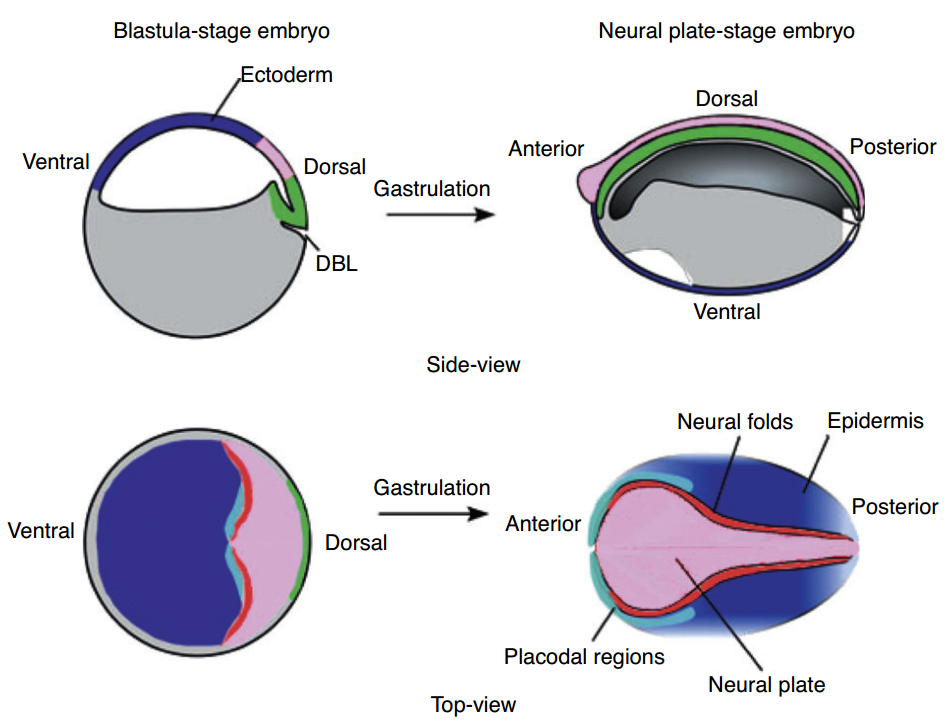
\includegraphics[width=\linewidth]{imgs/embryonic_origins_nervous_system.png}
	\caption{Embryonic origin of the neural system}
  	\label{fig:embrionicOriginNS}
\end{figure}

Figure \ref{fig:embrionicOriginNS}: the \textit{ectoderm} (blue/red in image) covers the outside of the embryon during \textit{gastrulation}.\footnote{Gastrulation is a phase early in the embryonic development of most animals, during which the single-layered \textit{blastula} is reorganized into a trilaminar ("three-layered") structure known as the \textit{gastrula}. These three germ layers are known as the ectoderm, mesoderm, and endoderm.} Ectodermal cells give rise to different derivatives depending on position along the dorsoventral (DV) axis of the embryo. The dorsal-most ectoderm (red) thickens to form the \textbf{neural plate}, a structure shaped like a tennis racquet with the head lying anteriorly. During a complex morphogenetic process called \textbf{neurulation}, the flat neural plate rolls up into a tube that sinks into the interior of the embryo and becomes overlain by epidermal ectoderm. This neural tube is the anlage of the central nervous system (CNS). As the neural plate folds and closes, neural crest cells detach from its lateral margins and migrate away, later condensing to form the major part of the peripheral nervous system (PNS).

\paragraph{The famous Spemann Organizer}

\begin{figure}
	\centering
  	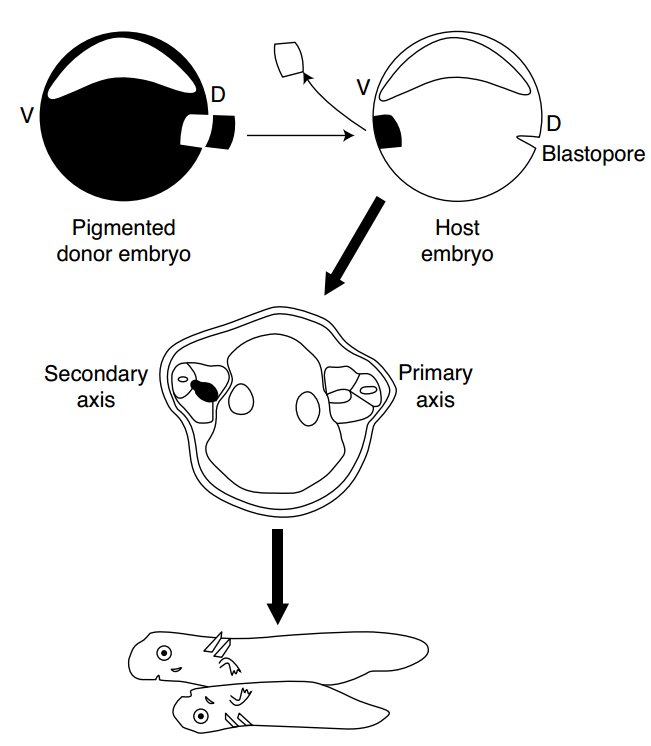
\includegraphics[width=0.5\linewidth]{imgs/spemann_organizer.png}
	\caption{Spemann Organizer Experiment}
  	\label{fig:spemannOrganizer}
\end{figure}

Figure \ref{fig:spemannOrganizer}: Tissue around the DBL\footnote{dorsal blastopore lip, where mesodermal cells start to involute during gastrulation} was removed from one embryo
(black) and placed into the ventral side of another (white). The transplanted DBL, if large enough, will cause a complete second dorsal axis to form on the host embryo, resulting in twinning. Cross section through the tadpoles shows that the second dorsal axis contains a complete nervous system. By using differently pigmented embryos, one can show that the majority of the nervous system in this new dorsal axis is not derived from the transplanted tissue, but rather from host tissue, fated to give rise to ventral tissues in the absence of a graft.

\paragraph{The default model for Neural Induction}
An important aspect of the default model for neural induction is that ectoderm will inherently (by default) form neural tissue unless it is exposed to antineuralizing signals.

\begin{figure}
	\centering
  	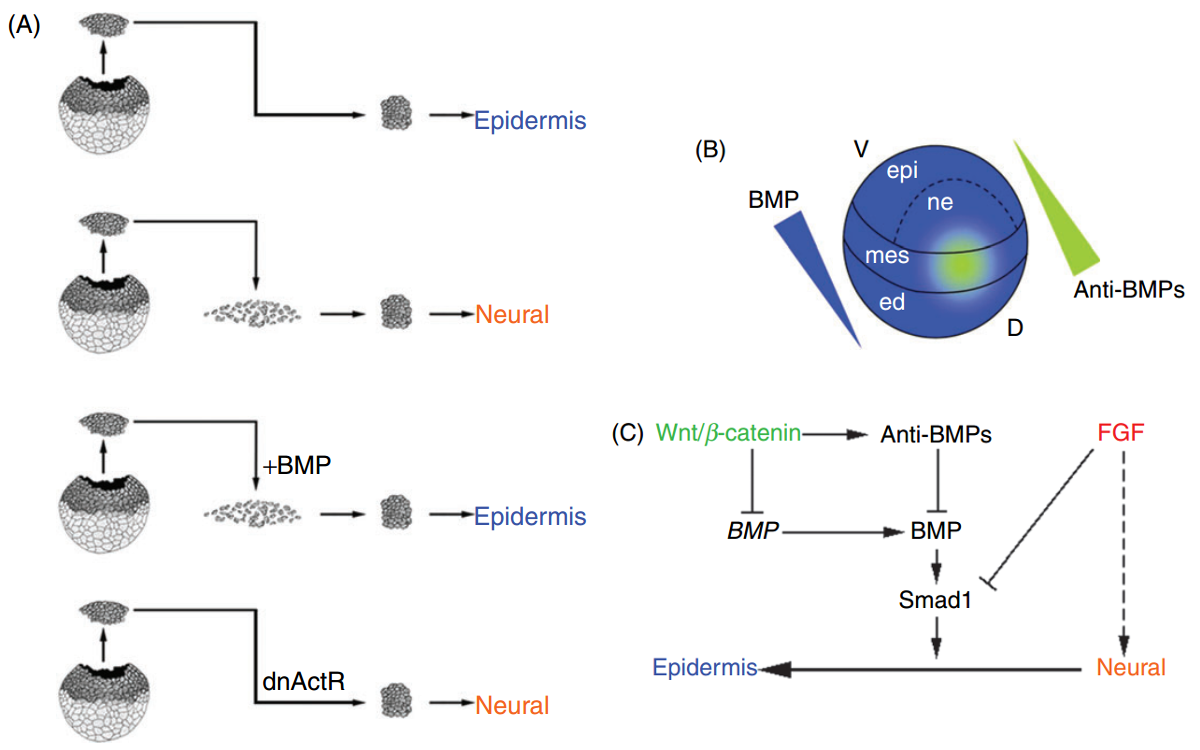
\includegraphics[width=\linewidth]{imgs/neural_induction.png}
	\caption{Default model for neural induction}
  	\label{fig:neuralInduction}
\end{figure}

Figure \ref{fig:neuralInduction}: Experiments in Xenopus embryos that led to the default model: culture of animal cap explant results in epidermis differentiation; dissociation for several hours followed by reaggregation of animal cap tissue results in neural induction; the presence of BMPs during dissociation prevents neural induction and promotes epidermis formation; the expression of a dominant-negative Activin receptor results in neural induction even without dissociation. BMPs induce epidermal fate and inhibit neural induction via Smad1 activity; BMP inhibitors act as neural inducers by blocking BMPs; FGFs act as neural inducers by counteracting Smad1 and via BMP-independent mechanisms; Wnt/$\beta$-catenin signaling predisposes ectoderm for neural induction by both preventing the transcription of Bmp genes and inducing the expression of BMP inhibitors.

\paragraph{Early Neural Patterning}
The neural plate is parcellated into subdivisions along the anterior-posterior (AP) and dorsalventral (DV) axes. This subdivision give rise to a multitude of different cell types in a spatially organized manner; these then become wired up in a stereotyped fashion and subserve distinct tasks in functional neural networks.

\subsubsection{Growth Cones and Axon Pathfinding}
\subsubsection{Cellular Determination}
\subsubsection{Neurogenesis and Migration}

\subsection{Excitability}
\subsection{Glia and more}
\subsection{Synapses}

\section{Systems Neuroscience}
\subsection{Somatosensory and Motor Systems}
\subsection{Visual System}
\subsection{Auditory \& Vestibular System}
\subsection{Circuits underlying Emotion}
\subsection{Learning in artificial and biological neural networks}

\section{Answers}
\subsection{Human \& Comparative neuroanatomy}

\subsubsection{Coronal section - I}
\begin{figure}[H]
	\centering
  	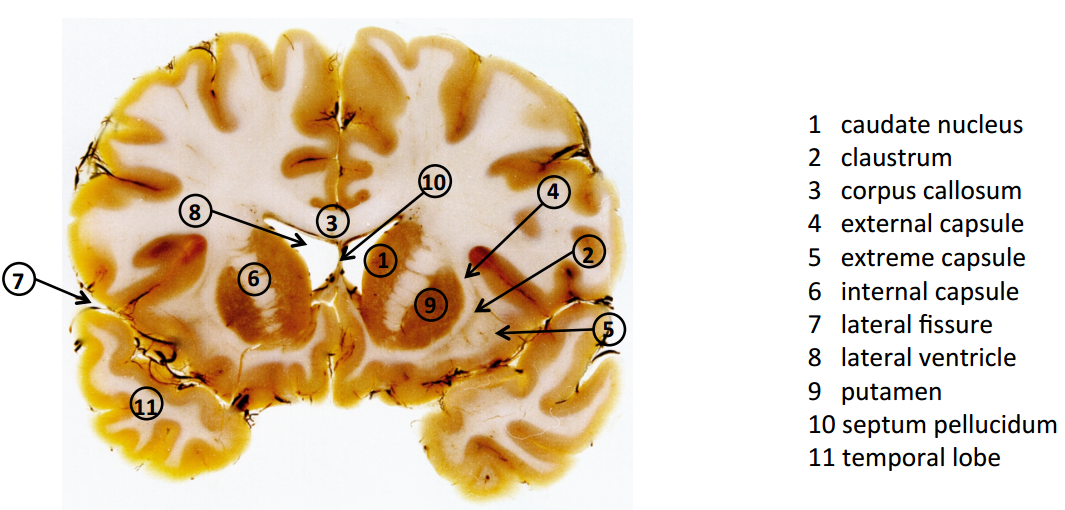
\includegraphics[width=\linewidth]{imgs/coronal-section-I-answer.png}
	\caption{Coronal section I}
  	\label{fig:coronalSectionI}
\end{figure}

\subsubsection{Coronal section - II}
\begin{figure}[H]
	\centering
  	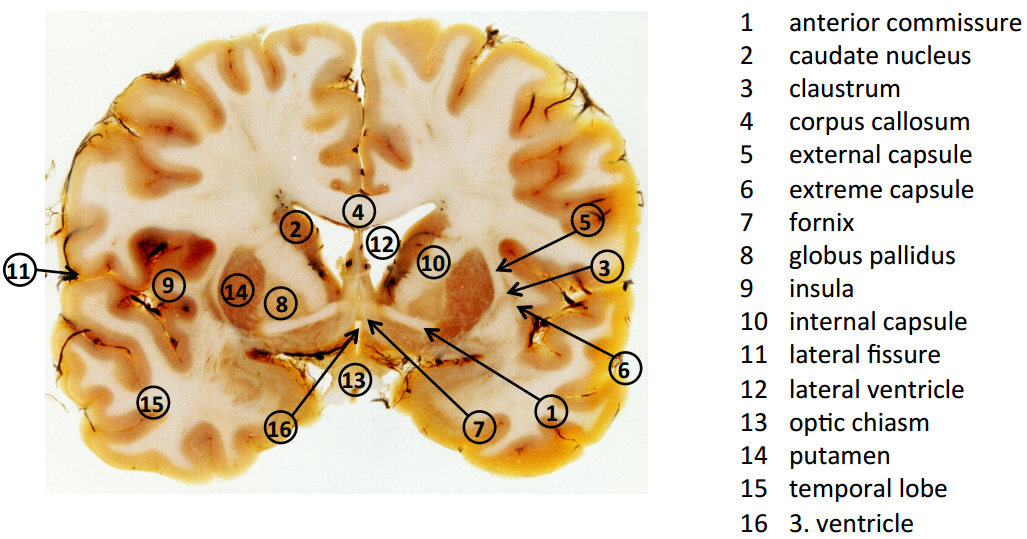
\includegraphics[width=\linewidth]{imgs/coronal-section-II-answer.png}
	\caption{Coronal section II}
  	\label{fig:coronalSectionI}
\end{figure}

\subsubsection{Coronal section - III}
\begin{figure}[H]
	\centering
  	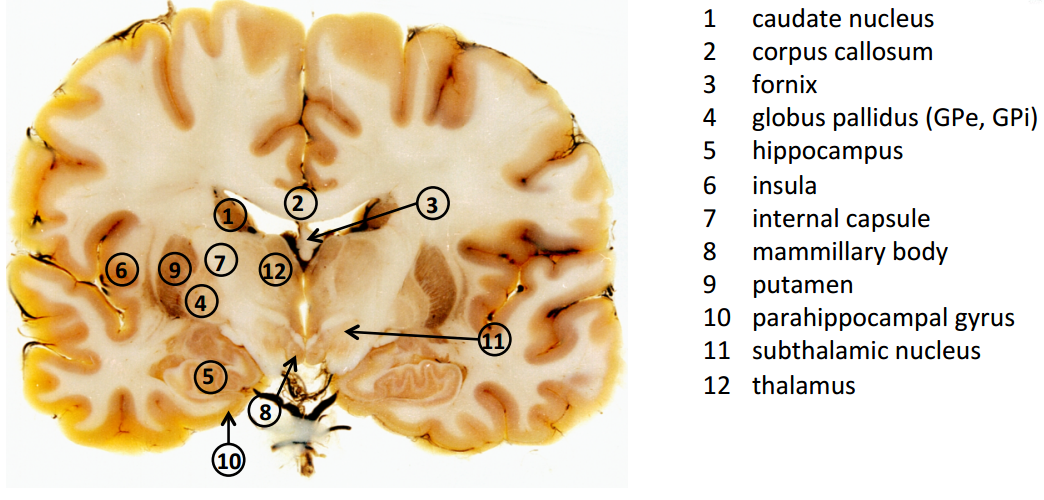
\includegraphics[width=\linewidth]{imgs/coronal-section-III-answer.png}
	\caption{Coronal section III}
  	\label{fig:coronalSectionI}
\end{figure}

\subsubsection{Coronal section - IV}
\begin{figure}[H]
	\centering
  	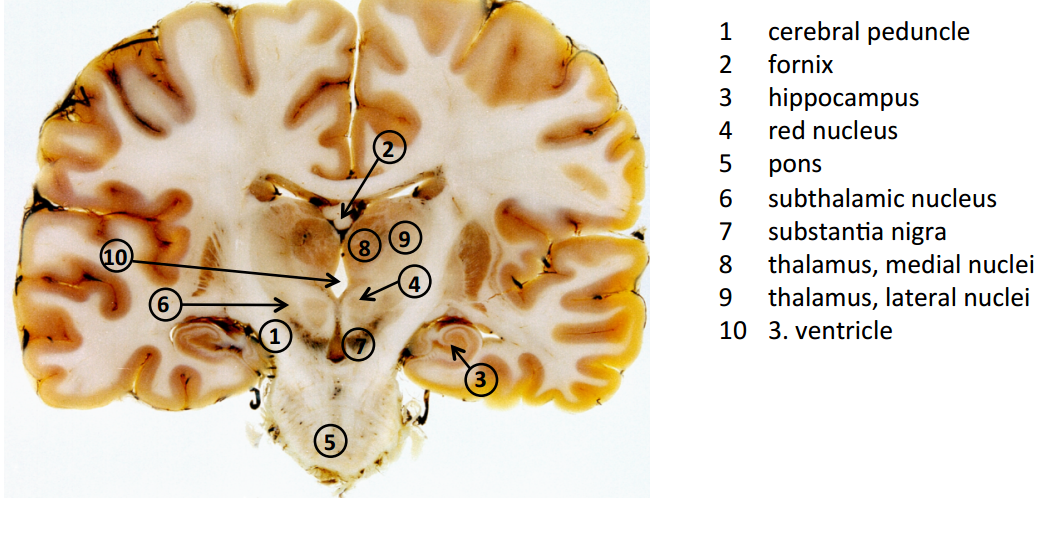
\includegraphics[width=\linewidth]{imgs/coronal-section-IV-answer.png}
	\caption{Coronal section IV}
  	\label{fig:coronalSectionI}
\end{figure}

\subsubsection{Horizontal section}
\begin{figure}[H]
	\centering
  	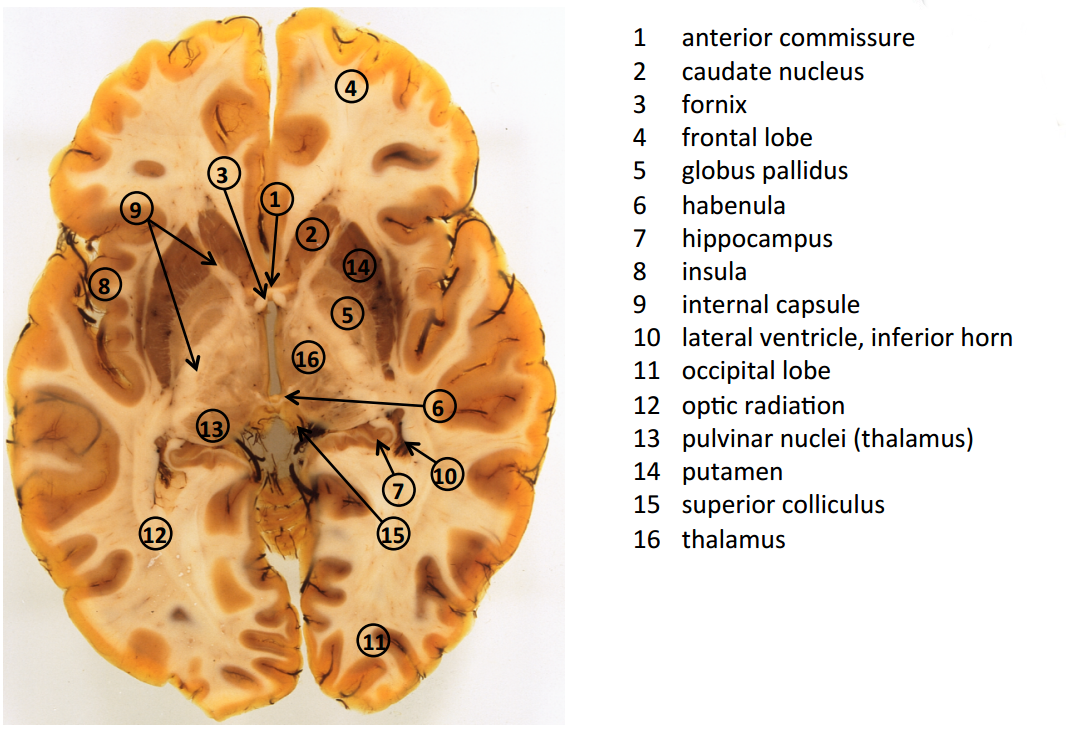
\includegraphics[width=\linewidth]{imgs/horizontal-section-answer.png}
	\caption{Horizontal section}
  	\label{fig:coronalSectionI}
\end{figure}

\newpage
\section{Previous Exams}
Note this answers were provided by students and were not verified by a teacher. Use them at your own risk.

\subsection{2013}
\paragraph{Q1. 5 methods (advantages + limitations) to label CNS neurons in rodent.}
\paragraph{Q2. Label 15 parts on a coronal slice (slice in which you see pons)}
\subparagraph{Describe how your project is related to some brain parts OR talk about the midbrain and its functional parts (+labelling a drawing of it).}
\paragraph{Q3. Chemical + electrical synapses}
\paragraph{Q4. A man with the “man who lost his body” documentary problem, how to test for his condition.}
\paragraph{Q5. Neurogenesis areas, labelling techniques, positive regulators and diseases associated with problems in neurogenesis.}
\paragraph{Q6. Bird auditory neuron behaviors, setup of the experiment with the bird and why is it important that the bird does not hear any external sounds.}

\subsection{2012}
\paragraph{Q1. Neuroanatomy}
\paragraph{Q2. Somatosensory}
\paragraph{Q3. Vision system}
\paragraph{Q4. Neural computation}
\paragraph{Q5. Brain development: neurogenesis}
\paragraph{Q6. Ion channel or synaptic transmission}

\subsection{2011}
\paragraph{Q1. Discuss the functions and structures of the hypothalamus as discussed in the lecture material.}
\subparagraph{Label 18 structures in 2 different coronal slices} see exercises.
\paragraph{Q2. Describe how DRG (dorsal root ganglion) sensory neurons development in comparison to motor neurons. How are cell boundaries formed in general and among the specific motor/sensory nerves}
\paragraph{Q3. Axon Guidance: what were sperry's findings that support the chemoaffinity hypothesis. What molecules are involved in this and how do they function.}
\paragraph{Q4. Describe from how sound is encoded neurally (from entering the ear to being perceived as sound in brain - complete pathway)}
\paragraph{Q5. Draw a flowchart for a typical neuroproteomics experiment}
\paragraph{Q6. Fill in the blank and multiple choice questions from Tobi's lecture: Who invented the term Neuro Engeneering? What is CMOS? Power consumption of brain. Synchronous logic is ubiquitous slide know physiologists friend photodiodes - how they are similar to retina CARVER MEAD}


\subsection{2010}
\paragraph{Q1. Auditory pathway}
\paragraph{Q2. Development of CNS and PNS}
\paragraph{Q3. Boundary building (one slide, different cell type)} ????
\paragraph{Q4. Pathfinding (Chemoaffinity, give 2 examples)}
\paragraph{Q5. Anatomy (hypothalamus, position and function)}
\paragraph{Q6. Neuromorphic engineering}

\subsection{2009}
\paragraph{Q1. Neuroanatomy: which of the 12 cranial nerves origin and/or end in the brainstem? What are their respective sensory, motor and /or vegetative functions ?(please describe in detail) Which nuclei of the cranial nerves are located in the mesencephalon?}
\paragraph{Q2. Auditory system: Describe differences between "conductive hearing loss" and "sensorineural hearing loss". Describe the classical test which is often used to determine between both forms of hearing loss. Describe biological causes and current treatments aids for such hearing impairments.}

\paragraph{Q3. Proteomics in neuroscience:}
\subparagraph{a. explain the term "proteome"}
\subparagraph{b. what are the benefits of measuring the proteome in addition to the genome?}
\subparagraph{c. Describe what a mass spectrometry is doing in principle.}
\subparagraph{d. How would you quantify proteins in a proteomic experiment? Please name and describe at least 2 proteomics technologies}
\subparagraph{e. Why is the proteome more complex compared to genome? Name and describe 3 reasons.}
\paragraph{Q4. Ion channels: What are the principal functions of dendrites, axon and nerves endings in the transcription of signals through the nervous system? Which types of ion channels are critical for the function of each of these 3 structures? Provide specific examples.}
\paragraph{Q5. Neural network: Explain the temporal and spatial network definition. Give an example for each network definition and describe how you can detect these networks in the brain.}
\paragraph{Q6. Neuromorphic engineering: Considering organizing principles used in biological retina explain (...)}

\subsection{2008?}
\paragraph{Q1. Describe the diencephalon and its major components according to the text "the brain in a nutshell"}
\paragraph{Q2. Compare structure and development of the cerebellum and the cortex}
\paragraph{Q3. What evidence did Sperry find that supports his chemoaffinnity hypothesis? Have Sperrys proposed "recognition molecules" been found? If yes name one example and describe what properties of this molecyles support its role as a recognition molecule}
\paragraph{Q4. Describe the structure of a voltage potassium channel. Explain the mechanisms that make the channel selective for only potassium ions.}
\paragraph{Q5. Describe three functional properties of neurons in v1 that are absent in the LGN. For each property describe in detail an experiment that illustrates it including the type of stimulus and the observed neural responses. Finally, choose one of these three properties and explain as presisely as possible how it can emerg at the cortical level.}
\paragraph{Q6. Which dynamic processes occur in single neuron and the local neural circuit during signal flow through a neural network? Name critical structural and functional aspects and discuss how they can be measured experimentally}

\subsection{2007}

\paragraph{Q1. Label each part of the brain, two coronal section, 18 areas.} see exercises.
\subparagraph{Describe the lobes of cortex, according to the handout.} 
\paragraph{Q2. Compare the cell migration to form the cortex and the migration in the peripheral neural system forming…} answer
\paragraph{Q3. About neurotrophic factor. What’s the experiment led to the finding of neurotrophic factor? Compare trophic and tropic factor.} answer	1
\paragraph{Q4. What’s the difference between ionotropic and metabotropic receptors?} Ionotropic receptors are made from proteins combined to form an ion channel. The neurotransmitter binds the receptor and open the channel for the ions going through. Ionotropic receptor have rapid changes with short duration. Metabotropic receptors are made of a single peptide and the neurotransmitter binds with a g-protein instead of the ion channel directly. It is need a second messenger to open the ion channel. Metabotropic receptors have slower response but with long duration.
\paragraph{Q5. Serotonin}
\paragraph{Q6. Insect eye}

\subsection{2006}
\paragraph{Q1. Label each part of the brain.} see exercises.
\subparagraph{Describe the components of midbrain according to the description in the shells of the brain}
\paragraph{Q2. Why the ion channel is selective to a ion with particular polarity, e.g. why the positive channel allows cations going through? List different ion channels in different part of the neuron: (1) axon, (2) axon terminal and (3) postsynaptic membrane}
\paragraph{Q3. How does cells differentiate in neural tube? How does cells differentiate in peripheral nervous system?}
\paragraph{Q4. What is the structure and function of myelinated nerve in PNS?}
\paragraph{Q5. Describe the structure and function of dopaminergic systems, the relation between the systems and psychology and neuropharmacology}
\paragraph{Q6. Visual system: describe the two columns in V1, and give out the definitions of them. What is the relation between this two columns and also between them and other part of visual system. Give out one experiment for testing of each column.}


\subsection{2005}
\paragraph{Q1. Draw the connectivity between motor cortex, thalamus, basal ganglia and cerebellum for motor control and show which connections are excitatory or inhibitory}
\subparagraph{Coronal view to fill with 16 names} see exercises.

\paragraph{Q2. Model organisms for understanding human brain development and function. Give three general advantages of these models. Compare in a table with advantages and disadvantages the models: Drosophila, C. Elegans, Zebrafish, Mouse. Give an example for each of how it helped understand the brain}

\paragraph{Q3. Two main route for cell death, detail differences}

\paragraph{Q4. Myelin: structure and function}

\paragraph{Q5. What are the two main modes of electrophysiological communication between neurons? Describe structure.}

\paragraph{Q6. Vision:}
\subparagraph{A. cites six roles for vision in insects}
\subparagraph{B. 1. what structural/functional differences between insect and human eyes 2. in what experiments are insects eyes worse or better than human eyes? 3. five share important features of insect and human eyes}
\subparagraph{C. 1. what is flow field? 2. draw the flow field perceived by a fly flying straight in a long corridor 3. what is ... field? ( i forgot the name oops) 4. draw pure rotation force field and its matched field filter}


\subsection{2004}
Some questions (especially number 6) are about subject not taught anymore during the first ZNZ introduction semester, so don't worry about them.

\paragraph{Q1. Describe the major formations involving the hippocampus in the associative cortex.}
\subparagraph{Coronal slices, 16 areas to be labelled} see exercises.
\paragraph{Q2. Structure and role of myelinating cells in the adult nervous system.}
\paragraph{Q3. Name some crucial functions of Neurotrophic factors.}
\paragraph{Q4. How is information transported in the nervous system? Explain features and function.}
\paragraph{Q5. In verterbrates the vision system has some special wiring pattern. What's special about it (as in, how is it different to olfaction)? Explain biological/physiological means in the development of vision.}
\paragraph{Q6. Imagine year 2020. Human genomics has advanced to the point where you not only can choose the gender and hair color of your child, but also apply specific changes to the visual system. Name 6 changes to the human visual system you would apply to your kid. Explain why you chose them and what physiological implications they would have.}

\newpage
\subsection{All Question - topics}

%%%%%%%%%%%%%%%%%%%%%%%%%%%%%%%%%%%%%%%%%%%%%%%%%%%%%%%%%%%%%%%%%%%%%%%%%%%%%%%%%%%%%%%%%%%%%
\subsubsection{Cytology}
\paragraph{Q1. What is the structure and function of a myelinated peripheral nerve?}
Structure: ???

The myelin in the peripherical nervous system is generated from Schwann cells. Myelin is a fatty substance (composed about 75\% of lipids, 20\% of proteins and 5\% of carbohydrates) that surrounds the axon of some nerve cells, in the PNS, the myelin is formed by many layers of schawnn cells membrane. The mainly function of a myelinated nerve is increase action potential conduction, that is, the message is delivered faster than an unmyelinated nerve. The myelin in peripheral nerve also provides a track along with a severed nerve can regrowth.

\paragraph{Q2. Myelin : structure and function}
Structure?

Myelin is a fatty substance (about 75\% of lipids, 20\% of proteins and 5\% of carbohydrates) that surround the axon of some nerve cells.
The maily function of the myelin is increase the action potencial conductancy, that is, to make the signal be propagated faster. In CNS the myelin is generated by olygodendrocytes and in the PNS by Schawnn cells.
In the PNS the myelin helps severed nerves to regrow, and unmyelinated and myelinated from CNS can't regenerate.

\paragraph{Q3. Structure and role of myelinating cells in the adult nervous system.}
Structure?

\paragraph{Q4. Serotonin}

\paragraph{Q5. Two main route for cell death, detail differences}

\paragraph{Q6. Proteomics in neuroscience:}
\subparagraph{a. explain the term "proteome"}
\subparagraph{b. what are the benefits of measuring the proteome in addition to the genome?}
\subparagraph{c. Describe what a mass spectrometry is doing in principle.}
\subparagraph{d. How would you quantify proteins in a proteomic experiment? Please name and describe at least 2 proteomics technologies}
\subparagraph{e. Why is the proteome more complex compared to genome? Name and describe 3 reasons.}

\paragraph{Q7. Two main routes for cell death, detail differences}

%%%%%%%%%%%%%%%%%%%%%%%%%%%%%%%%%%%%%%%%%%%%%%%%%%%%%%%%%%%%%%%%%%%%%%%%%%%%%%%%%%%%%%%%%%%%%
\subsubsection{Anatomy}
\paragraph{Q1. Describe the major formations involving the hippocampus in the associative cortex.} 
TODO:
associative: outside primary areas, It is essential for mental functions that are more complex than detecting primary sensory information
hippocampus: learning and memory
\paragraph{Q2. Label 2 coronal slices, 16/18 areas to be labelled} see exercises.
\paragraph{Q3. Mesencephalon: components \& nuclei (brain in a nutshell)}
TODO:
substantia nigra, superior colliculus (visual  and occulomotor reflexes), inferior colliculus (auditory tracts), crus cerebri, red nucleus
\begin{figure}[H]
	\centering
  	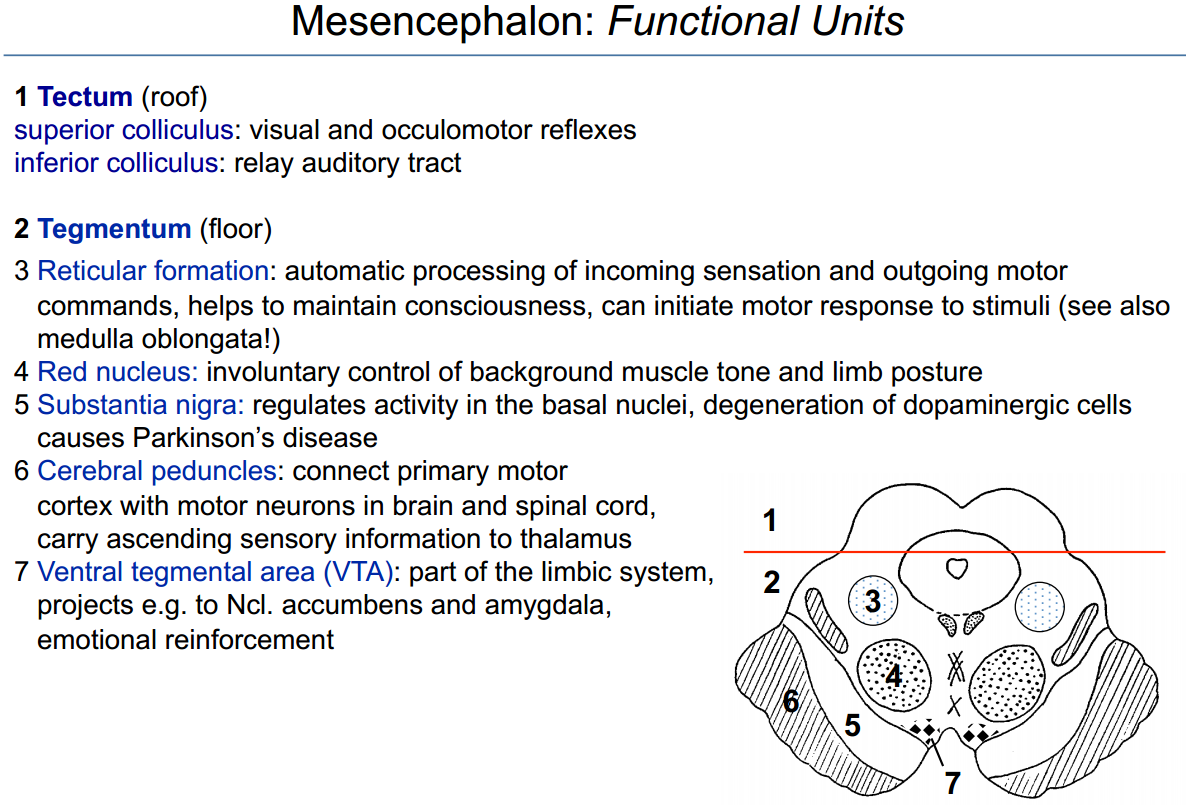
\includegraphics[width=\linewidth]{imgs/mesencephalon_answer.png}
\end{figure}
\paragraph{Q4. Motor activity structures and fibres}


\paragraph{Q5. Output structures and structures modulating output}

\paragraph{Q6. Draw the connectivity between motor cortex, thalamus, basal ganglia and cerebellum for motor control and show which connections are excitatory or inhibitory}


\paragraph{Q8. Describe the diencephalon and ist major components according to the text "the brain in a nutshell"}

\paragraph{Q9. Discuss the functions and structures of the hypothalamus as discussed in the lecture material.}

\paragraph{Q10. Anatomy (hypothalamus, position and function)}

\paragraph{Q11. Neuroanatomy: which of the 12 cranial nerves origin and/or end in the brainstem? What are their respective sensory, motor and /or vegetative functions? (please describe in detail). Which nuclei of the cranial nerves are located in the mesencephalon?}

\paragraph{Q12. Describe the lobes of cortex, according to the handout.} 

\paragraph{Q13. Describe the structure and function of dopaminergic systems, the relation between the systems and psychology and neuropharmacology}

\paragraph{Q14. Label 15 parts on a coronal slice (slice in which you see pons)}
\paragraph{Q15. Describe how your project is related to some brain parts OR talk about the midbrain and its functional parts (+labelling a drawing of it).}

%%%%%%%%%%%%%%%%%%%%%%%%%%%%%%%%%%%%%%%%%%%%%%%%%%%%%%%%%%%%%%%%%%%%%%%%%%%%%%%%%%%%%%%%%%%%%
\subsubsection{Development}
\paragraph{Q1. Name some crucial functions of Neurotrophic factors.}
Neurotrophic factors are a family of biomolecules that support the growth, survival and diferentiation of developing and mature cells.


\paragraph{Q2. How do different types of neurons differentiate in the neural tube?}

Developement: difference of development between sensory neurons from
DRG and Motor neurons in the spinal cord???
\paragraph{Q3. How do different types of neurons differentiate in the periphery?}

\paragraph{Q4. Example for migration}

\paragraph{Q5. Compare in a table with advantages and disadvantages the models: Drosophila, C. Elegans, Zebrafish, Mouse. Give an example for each of how it helped understand the brain}

\paragraph{Q6. Compare structure and development of the cerebellum and the cortex}

\paragraph{Q7. What evidence did Sperry find that supports his chemoaffinity hypothesis?}
The chemoaffinity hypothesis suggests that neurons make connections with their targets based on interactions with specific molecular markers. Sperry did the follow experiment: detached a frog eye, rotated it by 180 degrees, and then putted it back. When the axons rewired, the vision was rotated by 180 degrees. So, he create a hypothesis that there is a molecular tagging the axon grow.

\paragraph{Q8. Have Sperry’s proposed recognition molecules been found? If yes, name one example and describe what properties of this molecule supports it’s role as a recognition molecule.}
Yes, ...
EphA, Ephrin-A2...

\paragraph{Q9. Axon Guidance: what were sperry's findings that support the chemoaffinity hypothesis. What molecules are involved in this and how do they function.}

\paragraph{Q10. Development of CNS and PNS}

\paragraph{Q11. Pathfinding (Chemoaffinity, give 2 examples)}

\paragraph{Q12. Compare the cell migration to form the cortex and the migration in the peripheral neural system forming…}

\paragraph{Q13. What’s the experiment led to the finding of neurotrophic factor? Compare trophic and tropic factor.}

\paragraph{Q14. How does cells differentiate in neural tube? How does cells differentiate in peripheral nervous system?}

\paragraph{Q16. Neurogenesis areas, labelling techniques, positive regulators and diseases associated with problems in neurogenesis.}

\paragraph{Q17. 5 methods (advantages + limitations) to label CNS neurons in rodent.}

\paragraph{From class: What are neural stem cells?}
Neural stem cells are cells that can self­renew (maintenance and expansion). They can give rise to neurons and glia cells.

\paragraph{From class: How can adult neural stem cells be studied?} There are many ways to study adult neural stem cells, as radioation, retroviruses, genetic lineage tracing or even ablation of neurogenesis. The irradiation method has the disadvantage of produce an unsespecific effect of x-ray. 
...


\paragraph{From class: What influences Adult Neural Stem cells / Neurogenesis?}
In adults, the neurogenesis can be regulated for factors as voluntary exercise (running), enriched environment that increases neurogenesis or aging, stress, depression, drugs that decreases neurogenesis.

\paragraph{From class: What is the functional contribution of adult neural stem cells?}
There are some controversial results about the reason of neurogenesis in adults. The mainly (probably) functions are learning (hyppocampus and olfactory bulb), working memory and pattern separation (where two similar inputs are transformed in less similar inputs).

\paragraph{From class: Does adult neurogenesis occur in humans?}
Yes. However, there are just two areas where the adult neurogenesis occurs: SVZ (sub ventricular zone - olfactory bulb) and SGZ (sub granular zone - part of dentate gyrus of the hyppocampus).

\paragraph{From class: What it is a hope for degenerative diseases?} Therapy with neural stem cell transplantation. Neural stem cells can generate other type of cell and maybe regenerate some degenarated cells).

\paragraph{From class: How do axons move (mechanically)? Reorganization of microtubules in the growth cone how do axons navigate?}
The axons move using long range cues and short range cues. ...

\paragraph{From class: How to study basic principles of axonal pathfindig?} Stripe choice Assay 
1) midline studies
what is so interesting about the midline? Symetric environments but axons have to respond
differently e. g. on one side, the axon must be attracted to the midline, on the other side, it must find its target. comissure: are sites where axons cross the midline
topographic map: are systems in which groups of neurons in one tissue project their axons to another tissue in an organized arrangement such that spatial relationships are maintained
on the Professor: Dieter Zimmermann structure, expression and function on Versican: Versican: In our long­term basic research project we have been focusing on the large chondroitin sulfate proteoglycan versican and its putative role in the regulation of interactions between cells and their surrounding
extracellular matrix. This proteoglycan has been originally characterized by members of our group, partly in the USA and partly here at the Department of Pathology. Immunohistochemical, biochemical and cell biological studies of expression and function of different splice­variants of versican from our and other groups have provided strong evidence that versicans modulate cell proliferation and cell migration and control axonal growth during development. The marked re­expression of versicans in tumors of epithelial and non­epithelial origin has indicated a similar role of versican during tumor formation and progression.
contact attraction: Ephrin
contact repulsion: Versican
chemoattraction: Netrin
chemorepulsion: Semaphorin
guidepost cells

\paragraph{From class: Define the terms: sleep homoeostasis, circadian rhythm. Explain the physiological markers of each of these processes and describe their relevance and meaning.} sleep homeostasis: Homeostasis refers to regulatory mechanisms that maintain the constancy of the physiology of organisms. Sleep has a regulatory system enabling organisms to compensate for the loss of sleep (e.g. due to sleep deprivation) or surplus sleep (e.g by prolonging sleep in the morning or by napping). %from: $http://www.scholarpedia.org/article/Sleep_homeostasis#Definition$
Physiological markers: (here: regulated variable) $\rightarrow$ sleep intensity. The homeostatic mechanism regulates sleep intensity, while the circadian clock regulates the timing of sleep.
The intensity component of sleep is slow-wave activity (its level correlates positively with the threshold to arouse subjects or animals). Slow-wave activity is defined as spectral power of the electroencephalogram (EEG) in the frequency range of approximately 0.5 – 4.0 or 4.5Hz. Slow-wave activity increases as a function of the duration of prior wakefulness.

Circadian Rhythm: Repetitive event with a period length of about one day. from wiki: A circadian rhythm is a roughly 24 hour cycle in the physiological processes of living beings, including plants, animals, fungi and cyanobacteria. endogenous, entrainable
endogenous: built­in. self­sustained
markers: (in humans)  melatonin secretion by the pineal gland, core body temperature minimum, and plasma level of cortisol.

SCN
is located in the Hypothalamus
circadian pacemaker
two regions: VIP, DM
Every cell has its own clock?
How do they sync up?
1) Neuropeptides
2) electrical synapses
3) action potentials
Synaptic homeostasis hypothesis:
When we sleep, the connections — called synapses — weaken, allowing new information to
seep in.
This paper reviews a novel hypothesis about the functions of slow wave sleep—the synaptic
homeostasis hypothesis. According to the hypothesis, plastic processes occurring during
wakefulness result in a net increase in synaptic strength in many brain circuits. The role of
sleep is to downscale synaptic strength to a baseline level that is energetically sustainable,
makes efficient use of gray matter space, and is beneficial for learning and memory. Thus,
sleep is the price we have to pay for plasticity, and its goal is the homeostatic regulation of
the total synaptic weight impinging on neurons.
%http://www.sciencedirect.com/science/article/pii/S1087079205000420
%http://www.ncbi.nlm.nih.gov/pubmed/9374465
Transgenic Drosophila that expressed either luciferase or green fluorescent protein driven
from the promoter of the clock gene period were used to monitor the circadian clock in
explanted head, thorax, and abdominal tissues. The tissues (including sensory bristles in the
leg and wing) showed rhythmic bioluminescence, and the rhythms could be reset by light.
The photoreceptive properties of the explanted tissues indicate that unidentified
photoreceptors are likely to contribute to photic signal transduction to the clock. These
results show that autonomous circadian oscillators are present throughout the body, and they suggest that individual cells in Drosophila are capable of supporting their own
independent clocks. Gene identification: genetic screen $\rightarrow$ identification of Per1 $\rightarrow$ same gene also responsible for circadian clocks in humans

How is the mechanism of a circadian clock?
https://www.youtube.com/watch?v=1jkwUa6yTHw (ab 20 min)
How does the clock stay entrained with the environment?
light induced expression of clock genes in mammals: exclusively ocular entrainement, in drosophila, zebrafish all over the body Pharmacodynamics: drug targets and disease symptoms are cyclic
Does drug absorption vary with time?
ADME
Absorption. Distr.ibution. Metabolism. Excretion
Clock defects are linked with other brain disorders (affective disorders, depressive
disorders)

%%%%%%%%%%%%%%%%%%%%%%%%%%%%%%%%%%%%%%%%%%%%%%%%%%%%%%%%%%%%%%%%%%%%%%%%%%%%%%%%%%%%%%%%%%%%%
\subsubsection{Ion Channel}
\paragraph{Q1. Why is the ion channel selective to an ion with particular polarity, e.g. why the positive channel allows cations going through? List different ion channels in different part of the neuron: (1) axon, (2) axon terminal and (3) postsynaptic membrane}

Why: ??? \\
Ion channels are selectively permeable, that is, allow some types of ions going through. The selectivity usually uses the size and the charge of the ions.

\begin{itemize}
\item Axon ion channels: ion channels on axon are used to propagate the action potential. In unmyelinated axons, the action potential is propagated smoothly, however, in myelinated axon, there are ion channels only at nodes of ranvier, this way the action potential "jump" between nodes, and then is propagated faster.
\item Axon terminal ion channels: are the autoreceptors. Sometimes, the presynaptic cell release the neurotransmitters and they also bind with the ion channels on the presynaptic cell. This generates a feedback to the presynaptic cell.
\item Postsynaptic membrane ion channel: are the receptors. When the neurotransmitters are released on the synaptic cleft, they bind with the receptors (ion channels or g-proteins) and allow ions to cross the membrane.
\end{itemize}

\paragraph{Q2. Describe the structure of a voltage-gated potassium channel. Explain the mechanisms that make the channel selective for only potassium ions.}
A voltage-gate channel is a channel sensitive to the voltage gradient across the membrane. The voltage-gate potassium channel are selective for ions with the same charge and size of K+. The pore of potassium channel is negatively charged, attracting positive potassium. The channel has "filter" which is size-specific for potassium.

\paragraph{Q3. Draw a flowchart for a typical neuroproteomics experiment}

\paragraph{Q4. What are the principal functions of dendrites, axon and nerves endings in the transcription of signals through the nervous system? Which types of ion channels are critical for the function of each of these 3 structures? Provide specific examples.}

\paragraph{Q5. What’s the difference between ionotropic and metabotropic receptors?} Ionotropic receptors are made from proteins combined to form an ion channel. The neurotransmitter binds the receptor and open the channel for the ions going through. Ionotropic receptor have rapid changes with short duration. Metabotropic receptors are made of a single peptide and the neurotransmitter binds with a g-protein instead of the ion channel directly. It is need a second messenger to open the ion channel. Metabotropic receptors have slower response but with long duration.


%%%%%%%%%%%%%%%%%%%%%%%%%%%%%%%%%%%%%%%%%%%%%%%%%%%%%%%%%%%%%%%%%%%%%%%%%%%%%%%%%%%%%%%%%%%%%
\subsubsection{Synaptic Transmission}
\paragraph{Q1. How is information transported in the nervous system? Explain features and function.}
The information is transported either along a single neuron or between neurons. Along a single neuron with an action potential and between two neurons through synapses (chemical or electrical).
In chemical transmission, the presynaptic cell release vesicles that contains neurotransmitters in the synaptic cleft. Then, these neurotransmitters bind the receptors on the postsynaptic cell. The signal generated on the postsynaptic cell can be excitatory or inhibitory. If the signal is strong enough, the postsynaptic cell fires passing the information on.


\paragraph{Q2. Structural selectivity feature allowing cationic channel to conduct positive but not negative ions}



\paragraph{Q3. Transmission of neuronal signals: list ion channels critical for i) Axons ii) Dendrites (difference excitatory, inhibitory) and iii) Nerve Terminals}

\begin{itemize}
\item Axons: ion channels on axon are used to propagate the action potential. In unmyelinated axons, the action potential is propagated smoothly, however, in myelinated axon, there are ion channels only at nodes of ranvier, this way the action potential "jump" between nodes, and then is propagated faster.
\item dendrites: ion channel on dendrites are the receptors. When the neurotransmitters are released on the synaptic cleft, they bind with the receptors (ion channels or g-proteins) and allow ions to cross the membrane. The signal generated on the receptor cell can be excitatory or inhibitory. If the signal is strong enough, the postsynaptic cell fires passing the information on.
\item Nerve terminal ion channels: are the autoreceptors. Sometimes, the presynaptic cell release the neurotransmitters and they also bind with the ion channels on the presynaptic cell. This generates a feedback to the presynaptic cell.
\end{itemize}


\paragraph{Q4. Function of AP, resting potential, synaptic potential, channels for all these potentials}

\begin{itemize}
\item action potential: electrical signal produced on axon to boost the information flow in the neuron.	Main function is make the information going througth the axon, once the neuron is not naturally a good eletrical conductor.
\item resting potential: is the point of equilibrium wrt the ions to which the membrane is permeable. If the membrane is permeable just to one ion, then the resting potential will be equal to equilibrium potential for this ion. If the membrane is permeable to more than one ion, the resting potential is a value between all the individual equilibrium potential. The main function of the resting potential is be a threshold who indicates when a neuron fire or not.
\item synaptic potential: electrical signal associated with communication between neurons. The main function of the synaptic potential is allow transmission of information from one neuron to another.
\end{itemize}

\paragraph{Q5. What are the two main modes of electrophysiological communication between neurons? Describe structure.}
The two main modes of communication between neurons are chemical and electrical.
\begin{itemize}
\item chemical
\item electrical
\end{itemize}

\paragraph{Q6. Chemical + electrical synapses}

%%%%%%%%%%%%%%%%%%%%%%%%%%%%%%%%%%%%%%%%%%%%%%%%%%%%%%%%%%%%%%%%%%%%%%%%%%%%%%%%%%%%%%%%%%%%%
\subsubsection{Auditory System}
\paragraph{Q1. Describe from how sound is encoded neurally (from entering the ear to being perceived as sound in brain - complete pathway)}

\paragraph{Q2. Auditory pathway}

\paragraph{Q3. Describe differences between "conductive hearing loss" and "sensorineural hearing loss". Describe the classical test which is often used to determine between both forms of hearing loss. Describe biological causes and current treatments aids for such hearing impairments.}

\paragraph{Q4. Bird auditory neuron behaviors, setup of the experiment with the bird and why is it important that the bird does not hear any external sounds.}

%%%%%%%%%%%%%%%%%%%%%%%%%%%%%%%%%%%%%%%%%%%%%%%%%%%%%%%%%%%%%%%%%%%%%%%%%%%%%%%%%%%%%%%%%%%%%
\subsubsection{Sensory-Motor System}
\paragraph{Q1. Describe how DRG (dorsal root ganglion) sensory neurons development in comparison to motor neurons. How are cell boundaries formed in general and among the specific motor/sensory nerves}

\paragraph{Q2. Sensory inputs contribute to the production of locomotor patterns in three important ways. Identify these functions and illustrate them by means of clear examples.}

%%%%%%%%%%%%%%%%%%%%%%%%%%%%%%%%%%%%%%%%%%%%%%%%%%%%%%%%%%%%%%%%%%%%%%%%%%%%%%%%%%%%%%%%%%%%%
\subsubsection{Visual System}
\paragraph{Q1. Describe the two columns in V1, and give out the definitions of them. What is the relation between this two columns and also between them and other part of visual system. give out one experiment for testing of each column.}
In V1 we find two kind of columns: the orientation column and the ocular dominance column.
\begin{itemize}
\item orientation column: areas that selectively respond to specific orientation in the visual field. Experiment: present stimulli for an animal using different orientations, using a video camera record changes in light absorption. For each orientation stimullu use a color to combine all the recorded images. The combination will present a pattern as a pinwheel.
\item ocular dominance column: (also called ocular preference), some areas that are selective for one eye only. Experiment: close only the right eye from the animal and present stimulli to the left eye. Using a sensitive video camera record changes in light absorption that occur as the animal views the stimuli. After, close only the left eye of the animal and repeat the process. The difference between the two recorded images will appear with a stripped-shape, showing the ocular dominance.
\end{itemize}

The relation between the two columns is determined by the organization of the visual cortex. If you move the electrode tangentially through the cortex, you will find the ocular dominance column. However, if you move the electrode tangentially in the orthogonal direction you will find the orientation dominance.

Relation with other areas: ???


\paragraph{Q2. Describe three functional properties of neurons in area V1 that are absent in the Lateral Geniculate Nucleus. For each property describe in detail an experiment that illustrates it, including the type of stimulus and the observed neuronal responses. Finally, choose one these three properties and explain as precisely as possible how it can emerge at the cortical level.}

\begin{itemize}
\item binocular depth (stereopsis): in the V1 area, neurons have information about both eyes together, this way, they can be sensitive to the depth wrt the fixation point. Experiment: fix your finger in front of your eyes (with a distance about 10 centimeters. In an alternated way, open and close each eye (right eye closed and left open and vice-versa). You will see your finger in different positions. However, with both eyes open you see just one image.
\item orientation: Some V1 neurons are orientation selective - they respond strongly to lines, bars, or edges of a particular orientation (e.g., vertical). Experiment: an animal is fitted to focus the eyes on a screen, where oriented images will be projected. An extracellular electrode records the neuronal responses. We will see that some neurons will respond strongly for lines/bar/edges in specific orientation and will respond weakly (or even not respond at all) to other orientations.
\item direction (motion): Some V1 neurons are direction selective - they respond strongly to oriented lines/bars/edges moving in a preferred direction (e.g., vertical lines moving to the right). Experiment: the same experiment can be applied for direction. However, the oriented line/bar/edge will move for an specific direction this time. We will see that some neurons will respond strongly for lines/bar/edges moving in a specific direction and will respond weakly (or even not respond at all) to other directions.
\end{itemize} 

How binocularity emerge at the cortical level: each eye see the world from a slightly different point of view, so, objects that are before or after the fixation point are projected to noncorresponding points on the retinas. There are some neurons in V1 area that are maximally activated when the stimulus fall on noncorresponding points on the retina. They are the near cells and the far cells. The near cells discharge to disparities in front of the fixation point and the far cells discharge to disparities beyond the fixation point. The combination of these neurons contribute to the depth sensation.

\paragraph{Q3. In verterbrates the vision system has some special wiring pattern. What's special about it (as in, how is it different to olfaction)? Explain biological/physiological means in the development of vision.}

In visual system, there is a topographic map (the spatial arrangement in the retina is preserved in the primary visual cortex).

Specific targeting of projection neurons from the olfactory epithelium to the glomeruli
in the olfactory bulb is of course also needed but in the olfactory system encoding of
spatial information is not required. Rather, olfactory sensory neurons (OSNs) in the
olfactory epithelium that respond to the same odorant converge in the same
glomerulus of the olfactory bulb, forming a discrete rather than a topographic map
(Cho et al., 2009). Thus, the olfactory and the visual systems are wired
fundamentally differently (Figure 1A). Hence, it was not surprising that the molecular
mechanisms underlying the wiring of these two systems were found to be different.
from http://www.sciencedirect.com/science/article/pii/S0896627314010022

\paragraph{Q4. Imagine year 2020. Human genomics has advanced to the point where you
not only can choose the gender and hair color of your child, but also apply specific
changes to the visual system. Name 6 changes to the human visual system you would apply to your kid. Explain why you chose them and what physiological implications they would have.}

\begin{itemize}
\item add new subtype of cones to see other wavelength (much more colors and even infrared)
\item change the way how the ganglion axons exits retina, to avoid a blind spot.
\item add other subtypes of rod (to add color), this way, with low light the color will be still present.
\item 
\item
\item
\end{itemize}
%https://www.youtube.com/watch?v=T9HYPlE8xzc

\paragraph{Q5. Insect eye} 

\paragraph{Q6. Vision:}
\subparagraph{A. cites six roles for vision in insects}
\subparagraph{B. 1. what structural/functional differences between insect and human eyes 2. in what experiments are insects eyes worse or better than human eyes? 3. five share important features of insect and human eyes}
\subparagraph{C. 1. what is flow field? 2. draw the flow field perceived by a fly flying straight in a long corridor 3. what is ... field? ( i forgot the name oops) 4. draw pure rotation force field and its matched field filter}

%%%%%%%%%%%%%%%%%%%%%%%%%%%%%%%%%%%%%%%%%%%%%%%%%%%%%%%%%%%%%%%%%%%%%%%%%%%%%%%%%%%%%%%%%%%%%
\subsubsection{Learning and Memory}

\paragraph{Q1. Everything about declarative and nondeclarative memory:}
\subparagraph{short definitions}
\subparagraph{anatomical location}
\subparagraph{animal models}

\paragraph{Q2. Please give a definition of "classical conditioning" and explain in the terms US, CS and CR. Give at least two examples for rodent procedures of classical conditioning and specify for each of them what the US, CS and CR are.}

%%%%%%%%%%%%%%%%%%%%%%%%%%%%%%%%%%%%%%%%%%%%%%%%%%%%%%%%%%%%%%%%%%%%%%%%%%%%%%%%%%%%%%%%%%%%%
\subsubsection{Circuits underlying emotions}

\paragraph{Q1. Describe the potentiated startle reflex and underlying anatomical structures - fear}

%%%%%%%%%%%%%%%%%%%%%%%%%%%%%%%%%%%%%%%%%%%%%%%%%%%%%%%%%%%%%%%%%%%%%%%%%%%%%%%%%%%%%%%%%%%%%
\subsubsection{Neuromorphic engineering}

\paragraph{Q1. Differences in organizing principles between electronic and neural computation}

\paragraph{Q2. Illustrate neural computation principles by specific examples (e.g. retina), explain functional utility}

\paragraph{Q3. Neuromorphic engineering}

\paragraph{Q4. Considering organizing principles used in biological retina explain (...)}

%%%%%%%%%%%%%%%%%%%%%%%%%%%%%%%%%%%%%%%%%%%%%%%%%%%%%%%%%%%%%%%%%%%%%%%%%%%%%%%%%%%%%%%%%%%%%
\subsubsection{Neural networks}
\paragraph{Q1. Which dynamic process occur in single neurons and the local neural circuit during signal flow through a neuronal network? Name critical structural and functional aspects and discuss how they can be measured experimentally.}

\paragraph{Q2. Explain the temporal and spatial network definition. Give an example for each network definition and describe how you can detect these networks in the brain.}

\paragraph{Q3. Model organisms for understanding human brain development and function. Give three general advantages of these models. Compare in a table with advantages and disadvantages the models: Drosophila, C. Elegans, Zebrafish, Mouse. Give an example for each of how it helped understand the brain}


%%%%%%%%%%%%%%%%%%%%%%%%%%%%%%%%%%%%%%%%%%%%%%%%%%%%%%%%%%%%%%%%%%%%%%%%%%%%%%%%%%%%%%%%%%%%%
\subsubsection{Neural computation}
\paragraph{Q1. Fill in the blank and multiple choice questions from Tobi's lecture: Who invented the term Neuro Engeneering? What is CMOS? Power consumption of brain. Synchronous logic is ubiquitous slide know physiologists friend photodiodes - how they are similar to retina CARVER MEAD}

\paragraph{Q2. Describe the perceptron learning rule and example where it can be applied} 
Perceptron is suppervised learning
\newpage

\section{References}
The pictures used in this summary are from the class slide sets or internet, and belong to their respective owners. In the context of the summary they are used for educational purposes only.

\subsection{Molecular and Cellular Neuroscience}
\begin{itemize}
\item Building a central nervous system (Neuhauss and Jessberger)
\subitem Fundamental Neuroscience Part III, Chapters 13-16 (21)
\item Excitability (Müller)
\subitem Principles of Neural Science Part II, Chapter 5-7
\subitem Fundamental Neuroscience Part II, Chapter 5
\item Glia and more (Weber)
\subitem Fundamental Neuroscience Part II, Chapters 3, 12
\subitem Principles of Neural Science Part II, Chapter 4
\item Synapses (1/2) (Földy and Karayannis)
\subitem Fundamental Neuroscience Part II, Chapters 6-8 (Part 1) and 9-11 (Part 2)
\end{itemize}

\end{document}
